% Time-stamp: <2020-09-14 18:29:53 Romain>
% Beamer template for the Macro Stress-Testing Article
% August 2020
% Contact: Romain Lafarguette, rlafarguette@imf.org

%% ---------------------------------------------------------------------------
%% Preamble: Packages and Setup
%% ---------------------------------------------------------------------------
% Class 
\documentclass{beamer}

% Language
\usepackage[english]{babel}

% Font and encoding
\usepackage[utf8]{inputenc} % Input font
\usepackage[T1]{fontenc} % Output font
\usepackage{lmodern} % Standard LateX font
\usefonttheme{serif} % Standard LateX font

% Maths 
\usepackage{amsfonts, amsmath, mathabx, bm, bbm} % Maths Fonts

% Graphics
\usepackage{graphicx} % Insert graphics
\usepackage{subfig} % Multiple figures in one graphic
\graphicspath{{../output/}{../img/}}

% Colors
\usepackage{xcolor}
\definecolor{imfblue}{RGB}{0,76,151} % Official IMF color
\setbeamercolor{title}{fg=imfblue}
\setbeamercolor{frametitle}{fg=imfblue}
\setbeamercolor{structure}{fg=imfblue}
\setbeamercolor{page number in head/foot}{fg=imfblue}
\setbeamerfont{page number in head/foot}{size=\footnotesize}

% Tables
\usepackage{booktabs,rotating,multirow} % Tabular rules and other macros
\usepackage{pdflscape,afterpage} % Landscape mode and afterpage
\usepackage{threeparttable} % Split long tables
\usepackage[font=scriptsize,labelfont=scriptsize,labelfont={color=imfblue}]{caption}

% Import files
\usepackage{import}

% Appendix slides
\usepackage{appendixnumberbeamer} % Manage page numbers for appendix slides

% Bibliographies
\usepackage{natbib} % Author-year bibliography style

% A few macros: environments
\newenvironment{largeitemize}{\itemize\addtolength{\itemsep}{10pt}}{\enditemize}
\newenvironment{largeenumerate}{\enumerate\addtolength{\itemsep}{10pt}}{\endenumerate}
\newenvironment{wideitemize}{\itemize\addtolength{\itemsep}{30pt}}{\enditemize}
\newenvironment{wideenumerate}{\enumerate\addtolength{\itemsep}{30pt}}{\endenumerate}

% Define the footer with higher/lower adjustment
\defbeamertemplate{footline}{higher page number}
{
  \hfill
  \usebeamercolor[fg]{page number in head/foot}
  \usebeamerfont{page number in head/foot}  
  \thepage/\inserttotalframenumber\kern1em\vskip2pt %Change xxpt to
                                %lower/higher the footnote
}
\setbeamertemplate{footline}[higher page number]


% Remove navigation symbols and other superfluous elements
\setbeamertemplate{navigation symbols}{}
\setbeameroption{hide notes}
\setbeamertemplate{note page}[plain]
\beamertemplatenavigationsymbolsempty
\hypersetup{pdfpagemode=UseNone} % don't show bookmarks on initial view

% Institute font
\setbeamerfont{institute}{size=\footnotesize}
\DeclareMathSizes{10}{9}{7}{5}  

%% ---------------------------------------------------------------------------
%% Title info
%% ---------------------------------------------------------------------------
\title[]{FX Interventions Rules for Central Banks\\
A Risk-Based Framework}
\author[]{Romain Lafarguette \and Romain Veyrune}
\institute[]{IMF Monetary and Capital Markets Department \\ Central Bank Operations Division}

\date[]{\scriptsize September 2020 \\ \vspace{0.5cm} \scriptsize{\textit{The views
      expressed in this presentation do not necessarily represent the views of
      the IMF, its Executive Board, or IMF management} \vspace{-0.5cm}}}

\titlegraphic{
    \begin{figure}
    \centering
    \subfloat{{
\includegraphics[width=2cm]{imf_logo}}}%
    \end{figure}
}


% Insert the plan at each beginning of the section
\AtBeginSection[]
  {
     \begin{frame}
     \frametitle{Table of Contents}
     \tableofcontents[currentsection, hideothersubsections]
     \end{frame}
  }

%% ---------------------------------------------------------------------------
%% Title slide
%% ---------------------------------------------------------------------------
\begin{document}

\begingroup
\renewcommand{\insertframenumber}{}
\begin{frame}
  %\addtocounter{framenumber}{-1}
\maketitle
\end{frame}
\endgroup


%% ---------------------------------------------------------------------------
%% Framework
%% ---------------------------------------------------------------------------
\section{Conceptual Framework}

\begin{frame}
  \frametitle{Contributions}
  \begin{largeitemize}
    \item Design a  rule to \textbf{address tail-risks} related  to direct and indirect
exposures to exchange rate in the economy
    \item Provides guidance on \textbf{when} to intervene ("triggers")
    \item Appropriate for \textbf{floating exchange rate regimes} with FX
      macrofinancial risks (e.g. FX unhedged exposures,
      dollarization, etc.)
    \item Consistently target \textbf{FX risk} rather than arbitrary FX volatility/level threshold
    \item A \textbf{risk management framework} for central banks' financial
      stability mandate: aligned with \textbf{industry's best practices} in risk management
  \end{largeitemize}  
\end{frame}

\begin{frame}
  \frametitle{Key Messages}
  Foreign Exchange intervention rules should be:\\
  \medskip  
  \begin{largeitemize}
  \item \textbf{Adaptative}, depend on market conditions
  \item \textbf{Objective}, anchored to a risk tolerance level
    rather than an aribtrary FX level threshold
  \item Capture FX \textbf{non-linearities and asymmetries} between appreciation and
    depreciation
  \item Be easily \textbf{operationalizable}, and \textbf{financially viable}\\
  \end{largeitemize}
\medskip  
We propose an FX intervention rule based on \textbf{Conditional Value-at-Risk}  
\end{frame}

\begin{frame}
  \frametitle{Concept: Value-at-Risk FXI Rule}
  \begin{largeitemize}
    \item Rather than using a fixed volatility rule (e.g. intervene if daily
      exchange rate varies by more than 2\%)
    \item Use a \textbf{risk-based rule}: intervene when the daily exchange
      rate log-returns fall within the
      tails of the conditional distribution
    \item Measure the tail-risk via the concept of \textbf{Value-at-Risk} (the
      conditional quantile of the log returns distribution) 
    \item The conditional distribution is estimated daily with a standard
      financial GARCH model and \textbf{varies with market conditions}
    \item The central bank decides on the \textbf{risk tolerance}:
      e.g. intervene in the tail at 1\%, 5\%, 10\%, etc.
  \end{largeitemize}
\end{frame}

\begin{frame}
  \frametitle{VaR FXI Rule}
    \makebox[\linewidth]{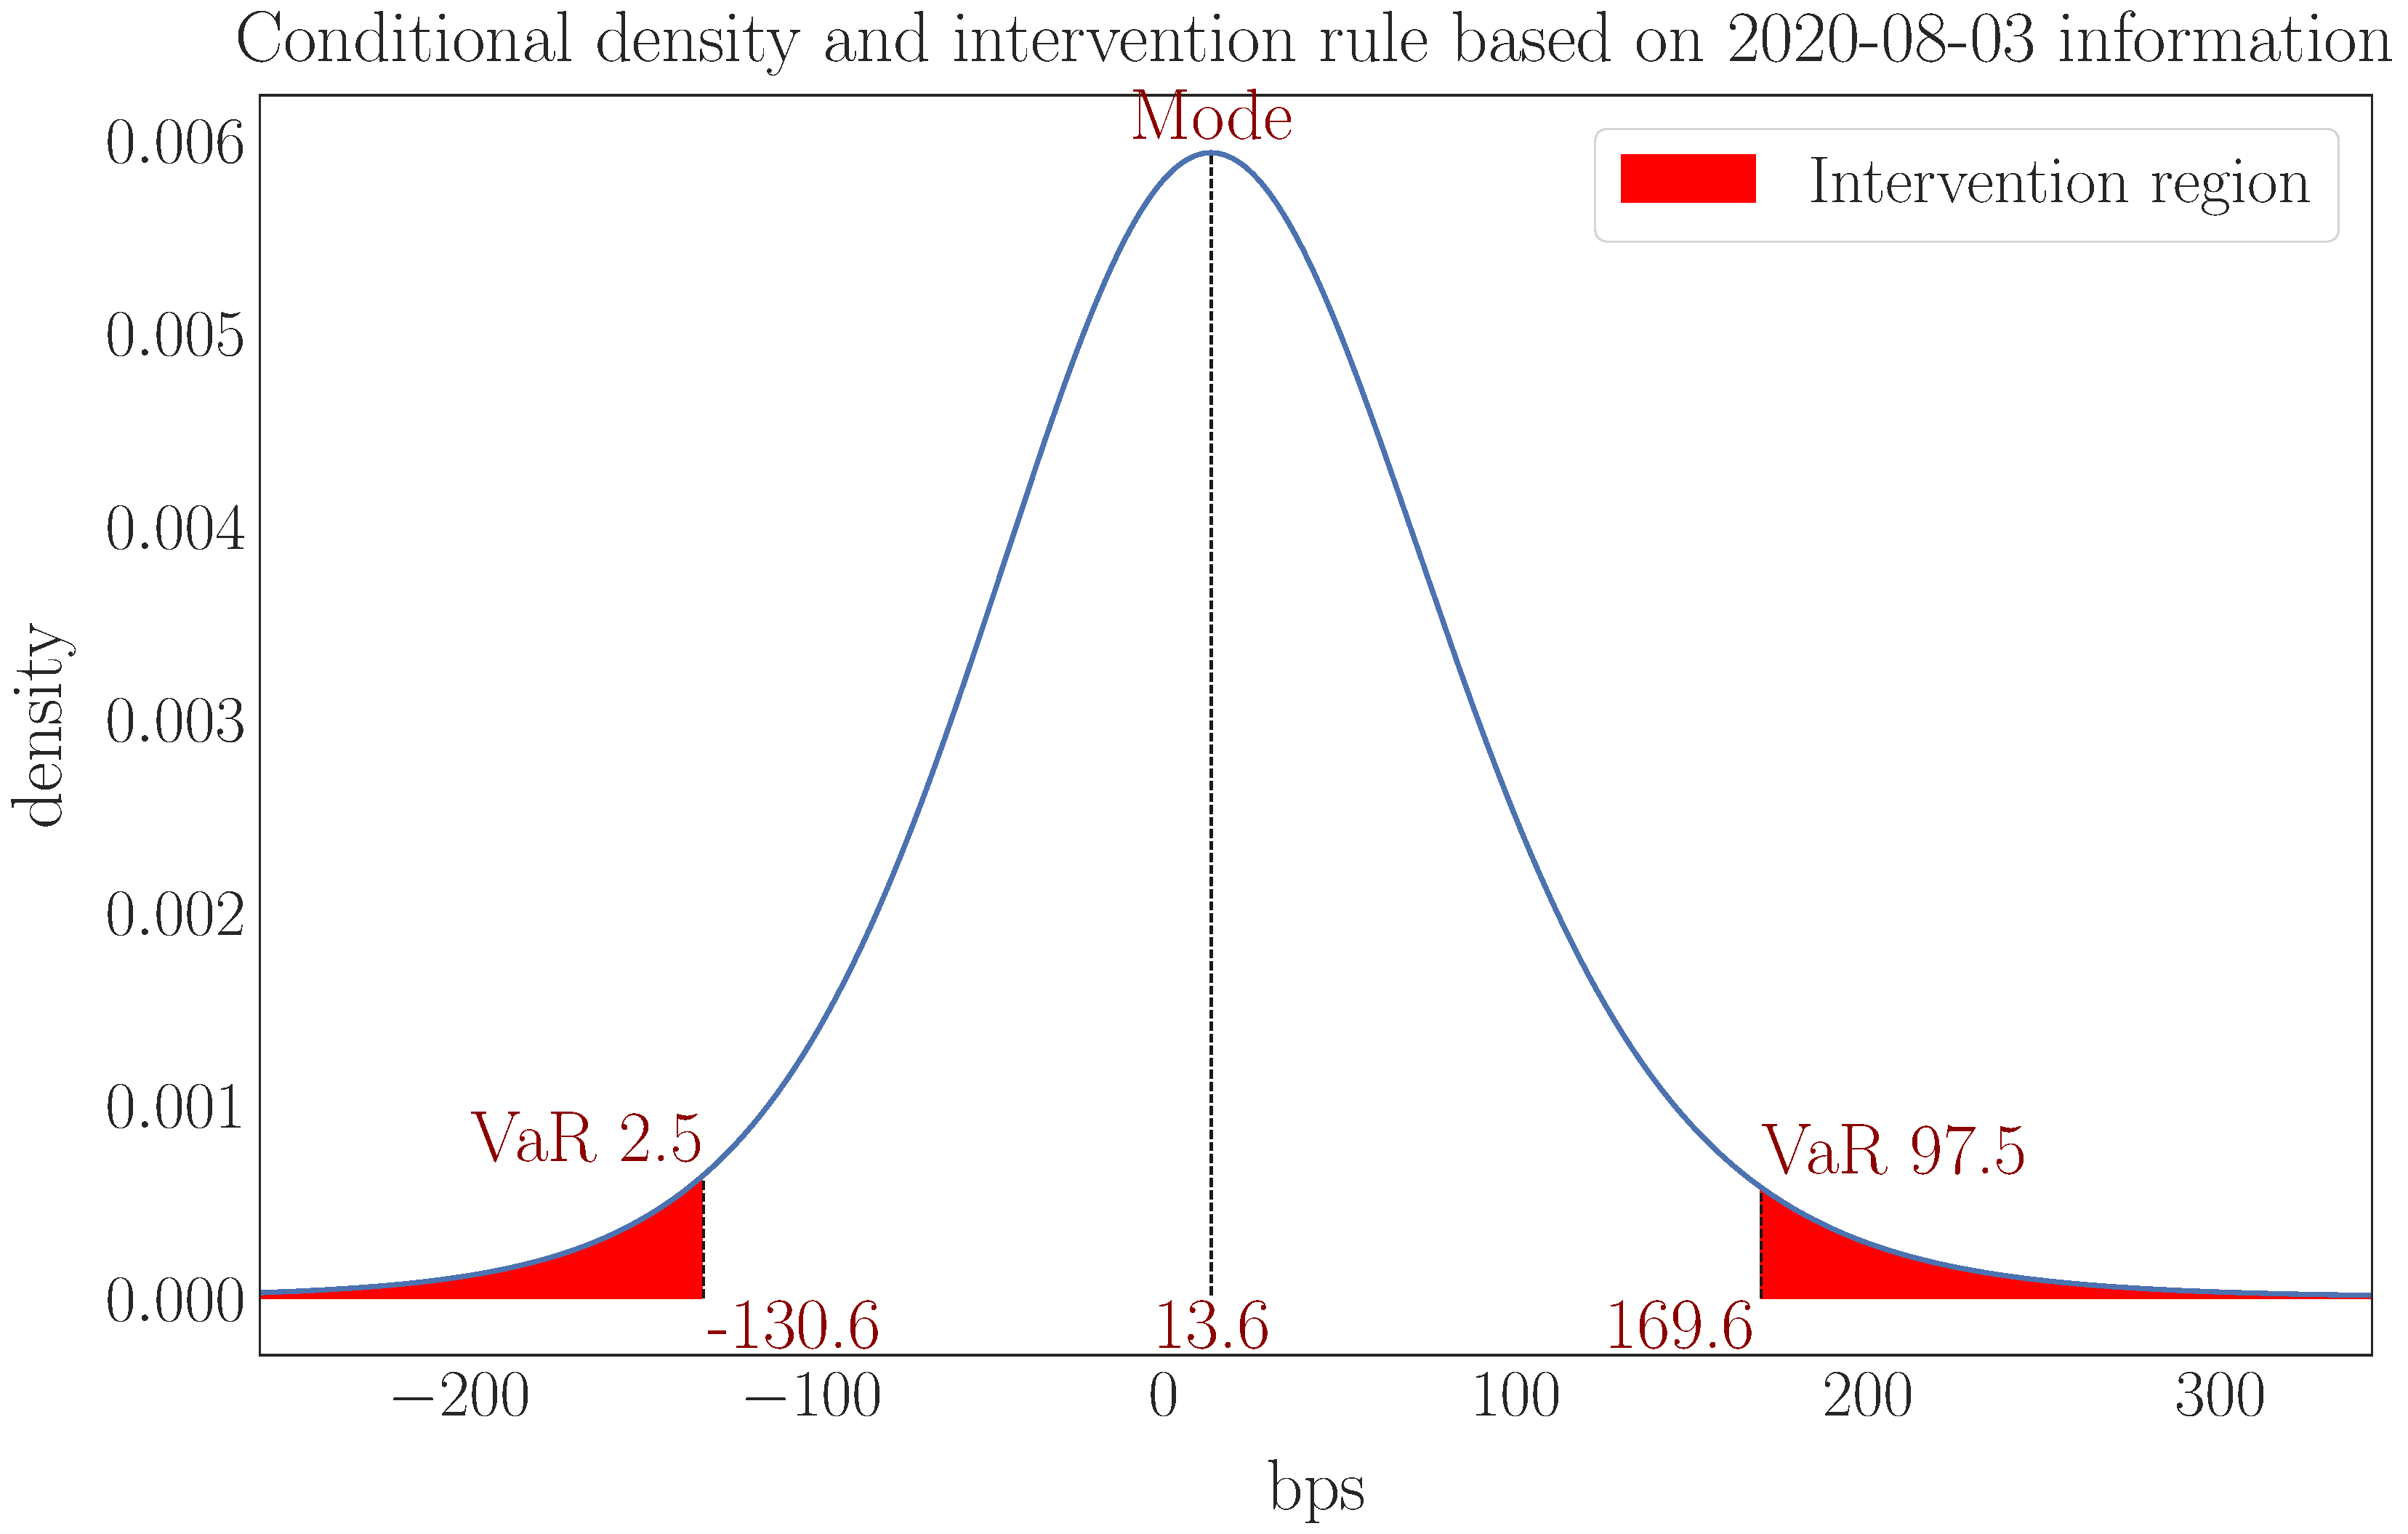
\includegraphics[width=\paperwidth]{var_rule.pdf}}
\end{frame}

\begin{frame}
  \frametitle{A Risk-Management Approach to FX Interventions}
  \begin{largeitemize}    
  \item Tail-risks hedge not always available: \textbf{incomplete markets}
    \item \textbf{The central bank is transferring FX risk from the market to
      its balance sheet}. It buys a risky asset (FX) and issues a risk-free asset
      (local currency)    
    \item Provide a \textbf{public good} to address market failure. Leave a
      fix share of risk for the market to hedge 
    \item Risk tolerance should depend on the \textbf{macrofinancial risk} (FX
      unhedged exposures from residents, dollarization, etc.) 
    \item The financial stability mandate of the central bank is properly
      formalized and quantified via VaR metric
  \end{largeitemize}  
\end{frame}

\begin{frame}
    \frametitle{Main Features}
  \begin{largeenumerate}
  \item This rule allows flexible exchange rate to act as a \textbf{shock absorber}:
    provides more flexibility in crisis time.
  \item No excessive interventions in crisis time which are often ineffective
    and costly (exhaust central bank FX reserves)
  \item Doesn't provide a free insurance to the market: avoid \textbf{moral
      hazard} and foster the \textbf{development of hedging market}
  \item Adaptative rule prevent \textbf{market manipulation and windfall effects}
  \item This rule guarantees that the interventions will occur with a \textbf{fixed
        frequency} over the medium term => \textbf{budget neutrality} with
      symmetric risk preference
  \item \textbf{Financially optimized}: always buy/sell at the best price
  \end{largeenumerate}  
\end{frame}


\begin{frame}
  \frametitle{Operational Implementation}
  \begin{largeitemize}
  \item \textbf{Standard data requirements}, easily accessible for a central
    bank, can be customized
  \item Parsimonious GARCH model featuring \textbf{embedded heteroskedasticity},  \textbf{asymmetries}
    (appreciation/depreciation), \textbf{non-linearities} (exponential
    volatility) and parametric \textbf{density forecasting}    
  \item We created a Python wrapper, \textbf{free and open-source}: estimation, forecasting,
    out-of-sample evaluation, benchmarking, etc. Results are \textbf{fully replicable}
  \item Can be readily used by central banks and deployed during Technical Assistance missions
  \end{largeitemize}
\end{frame}


\begin{frame}
  \frametitle{Challenges}
  \begin{largeitemize}
      \item Some central banks might be reluctant to use a VaR-rule: more
        difficult to communicate to the public
      \item However, FXI occur on the wholesale FX market, where market
        participants are fully aware of the VaR concept
    \item Some policy markers might prefer to keep discretion
    \item Trade-off: a transparent rule anchors better market expectations,
      maximize efficiency and isolate the central bank for political pressures    
  \end{largeitemize}
\end{frame}

\begin{frame}
  \frametitle{Usages}    
  \begin{largeenumerate}
    \item Determine FX Intervention triggers
    \item Conduct market monitoring and provide policy guidance
    \item Benchmark FX interventions, including discretionary interventions
    \end{largeenumerate}
    
    \bigskip
    
  \begin{largeitemize}
    \item We present below an application of the toolkit to the Mexican Peso, based on publicly
      available data
    \item More than 4500 daily observations, from 2009 to 2018, with Bank of
      Mexico (public) FX interventions, mostly concentrated in 2009 and 2016
    \end{largeitemize}
    
\end{frame}


%% ---------------------------------------------------------------------------
%% Model
%% ---------------------------------------------------------------------------
\section{Model}

\begin{frame}
  \frametitle{Specification}
\begin{largeitemize}  
\item Non-linear, Exponential GARCH (EGARCH) model 
\item The dependent variable is the FX log-returns, $r_t = \log(\frac{e_t}{e_{t-1}})$, where
$e_t$ is the bilateral market exchange rate against the major currency
(e.g. USD)
\item \textbf{Drift AR-X(1):} $r_{t+1} = \alpha_d +
  \rho r_t + \beta X_{t+1} + \epsilon_{t-1}$\\  
\item \textbf{Exponential volatility:} $\log \sigma_{t+1}^{2} = \omega + \beta
g(r_t)$ where $g(r_t) = \alpha_v r_t + \gamma(|r_t|-\mathbb{E}|r_t|)$

\item \textbf{Error term distribution} $\epsilon_t = \sigma_t \varepsilon_t
  \ , \varepsilon_t \sim \text{TSK}(0, 1,\nu)$\\
  
\item The forecasted conditional probability distribution function is defined as:
      \begin{equation*}
        \hat{f}(r_{t+1} | r_{t}, X_{t+1}) = \text{TSK}(\hat{r}_{t+1},
        \hat{\sigma}_{t+1}^{2}, \hat{\nu})
      \end{equation*}      
\end{largeitemize}
\end{frame}

% Estimation
\begin{frame}{Estimation}
\begin{largeitemize}
\item The GARCH estimation is standard and done with maximimum likelihood
 \item Selection of parameters is done via AIC/BIC criteria.    
  \item Our Python package allows to flexibly select:
    \begin{itemize}
    \item The set of exogeneous regressors
    \item The number of lags
    \item The volatility specification (exponential, RiskMetric, standard GARCH,
      etc.)
    \item The distribution family of the error-terms (Gaussian,
    Student, Tskew, Generalized Gaussian, etc.)  
      \end{itemize}    
\end{largeitemize}
\end{frame}

\begin{frame}{Exogeneous Regressors}
  \begin{largeenumerate}
  \item \textbf{FX microstructure}: FX bid-ask spread (averaged over the day)
  \item \textbf{CIP}: daily interest rate differential with the US Libor 
  \item \textbf{Hedging costs}: one-month forward exchange rate
  \item \textbf{Past policy interventions}: lagged amount of central bank FX intervention 
  \item \textbf{Global risk sentiment}: The VIX, implied volatility on the S\&P 500 
  \item \textbf{Global FX factor}: The EURUSD exchange rate
  \end{largeenumerate}
 
\end{frame}


\begin{frame}{Regression Table}
\setlength\tabcolsep{2pt}  % default value: 6pt
\tiny  %%  command to change the font size
\begin{tabular}{llllll}
\toprule
{} & Microstructure &       CIP & Dollar move & Risk Appetite &  Baseline \\
\midrule
Intercept                       &       -2.33*** &     -2.29 &       -1.84 &         -2.55 &     -1.63 \\
Lag FX log returns              &       -0.07*** &     -0.08 &    -0.08*** &      -0.08*** &  -0.08*** \\
Bid ask abs                     &           5.71 &     24.39 &      -35.66 &         -2.42 &      3.23 \\
Min max abs                     &       35.56*** &     34.63 &       34.32 &        34.55* &     26.21 \\
Forward points first difference &       23.29*** &  17.79*** &    26.44*** &       19.8*** &  19.44*** \\
Interbank rate vs Libor         &                &  33.61*** &    39.32*** &      34.75*** &  33.86*** \\
EURUSD log returns              &                &           &    -0.14*** &      -0.17*** &  -0.16*** \\
VIX first diff                  &                &           &             &      15.66*** &  15.37*** \\
FX intervention dummy lag       &                &           &             &               &      2.23 \\
Oil prices log returns          &                &           &             &               &  -0.02*** \\
Omega                           &        0.13*** &      0.13 &     0.12*** &       0.11*** &   0.12*** \\
Alpha                           &        0.17*** &     0.17* &     0.16*** &       0.16*** &   0.15*** \\
Gamma                           &        0.07*** &   0.06*** &     0.06*** &       0.05*** &   0.05*** \\
Beta                            &        0.98*** &   0.99*** &     0.99*** &       0.99*** &   0.99*** \\
Nu                              &        8.33*** &   8.66*** &     8.92*** &       8.71*** &   8.54*** \\
Lambda                          &        0.08*** &      0.07 &        0.09 &         0.07* &   0.08*** \\
R2                              &          5.8 \% &     6.7 \% &      10.4 \% &        27.3 \% &    27.6 \% \\
R2 adjusted                     &          5.8 \% &     6.6 \% &      10.4 \% &        27.2 \% &    27.5 \% \\
Number of observations          &           5986 &      5986 &        5682 &          5682 &      5680 \\
Significance *10\%, **5\%, ***1\%  &                &           &             &               &           \\
\bottomrule
\end{tabular}

\normalsize
\end{frame}

\begin{frame}{Formalization of the Intervention Rule}
  \begin{largeitemize}
    \item Consider the estimated conditional distribution of the exchange rate log
      returns $r_t$ defined as
      \begin{equation*}
      \mathbb{P}[r_t \leq x] = \int_{-\infty}^{x}\hat{f}(r_t | r_{t-1}, X_t)
      dr_t        
      \end{equation*}
    \item The Conditional Value-at-Risk at threshold $\tau$ is simply defined as
      the conditional $\tau$-quantile
      \begin{equation*}
      Q(r_t, \tau) \equiv  \mathbb{P}[r_t
      \leq Q(r_t, \tau)] = \tau, \ \text{for} \ \tau \in (0,1)
      \end{equation*}        
    \item The FXI intervention rule is a simple boolean rule, based on two
      risk-thresholds ($\underline{\tau}, \overline{\tau}$), for depreciation
      and appreciation, potentially risk-symmetric ($\overline{\tau} = 1 - \underline{\tau}$)
      \begin{equation*}
\mathbbm{1} \left[ \{r_t \leq \ Q(r_t, \underline{\tau})\} \cup \{r_t > \
  Q(r_t, \overline{\tau})\} \right]
      \end{equation*}                
  \end{largeitemize}
  
\end{frame}

\begin{frame}
\frametitle{Dynamics of the Mexican Peso against USD}
    \makebox[\linewidth]{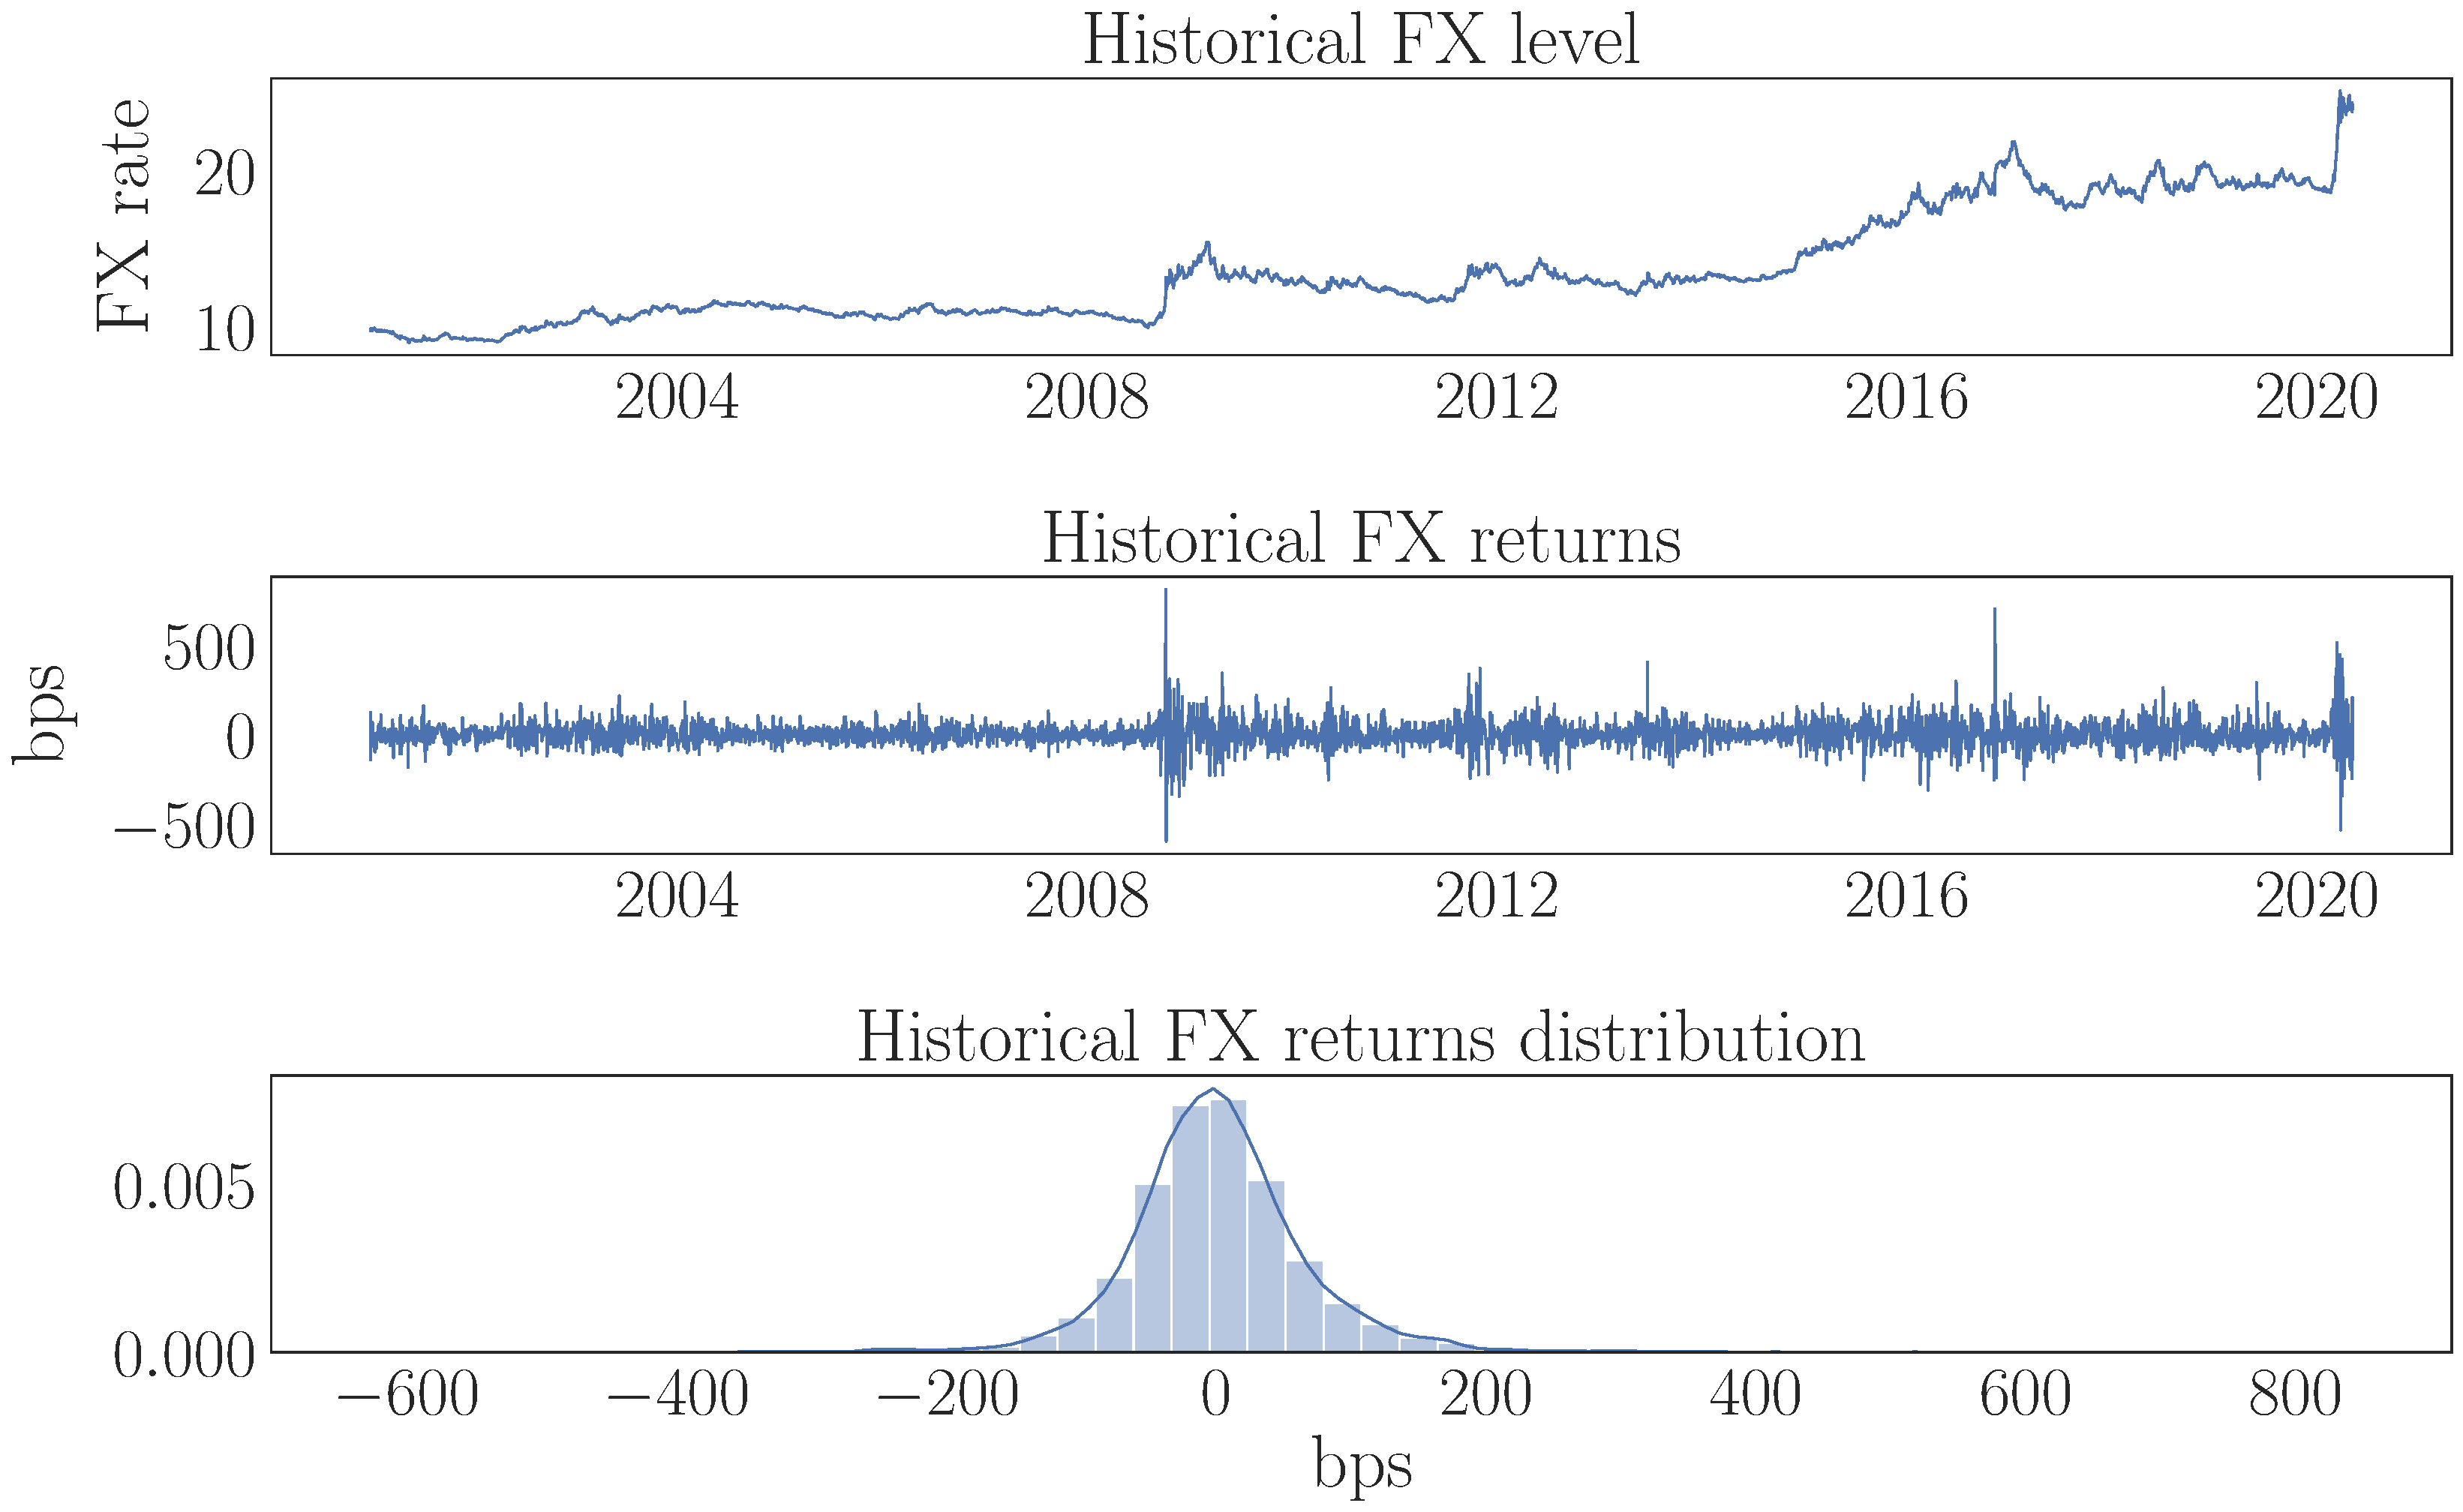
\includegraphics[width=\paperwidth]{descriptive_plot.pdf}}
\end{frame}

\begin{frame}
\frametitle{Conditional In-Sample Volatility of the Mexican Peso}
    \makebox[\linewidth]{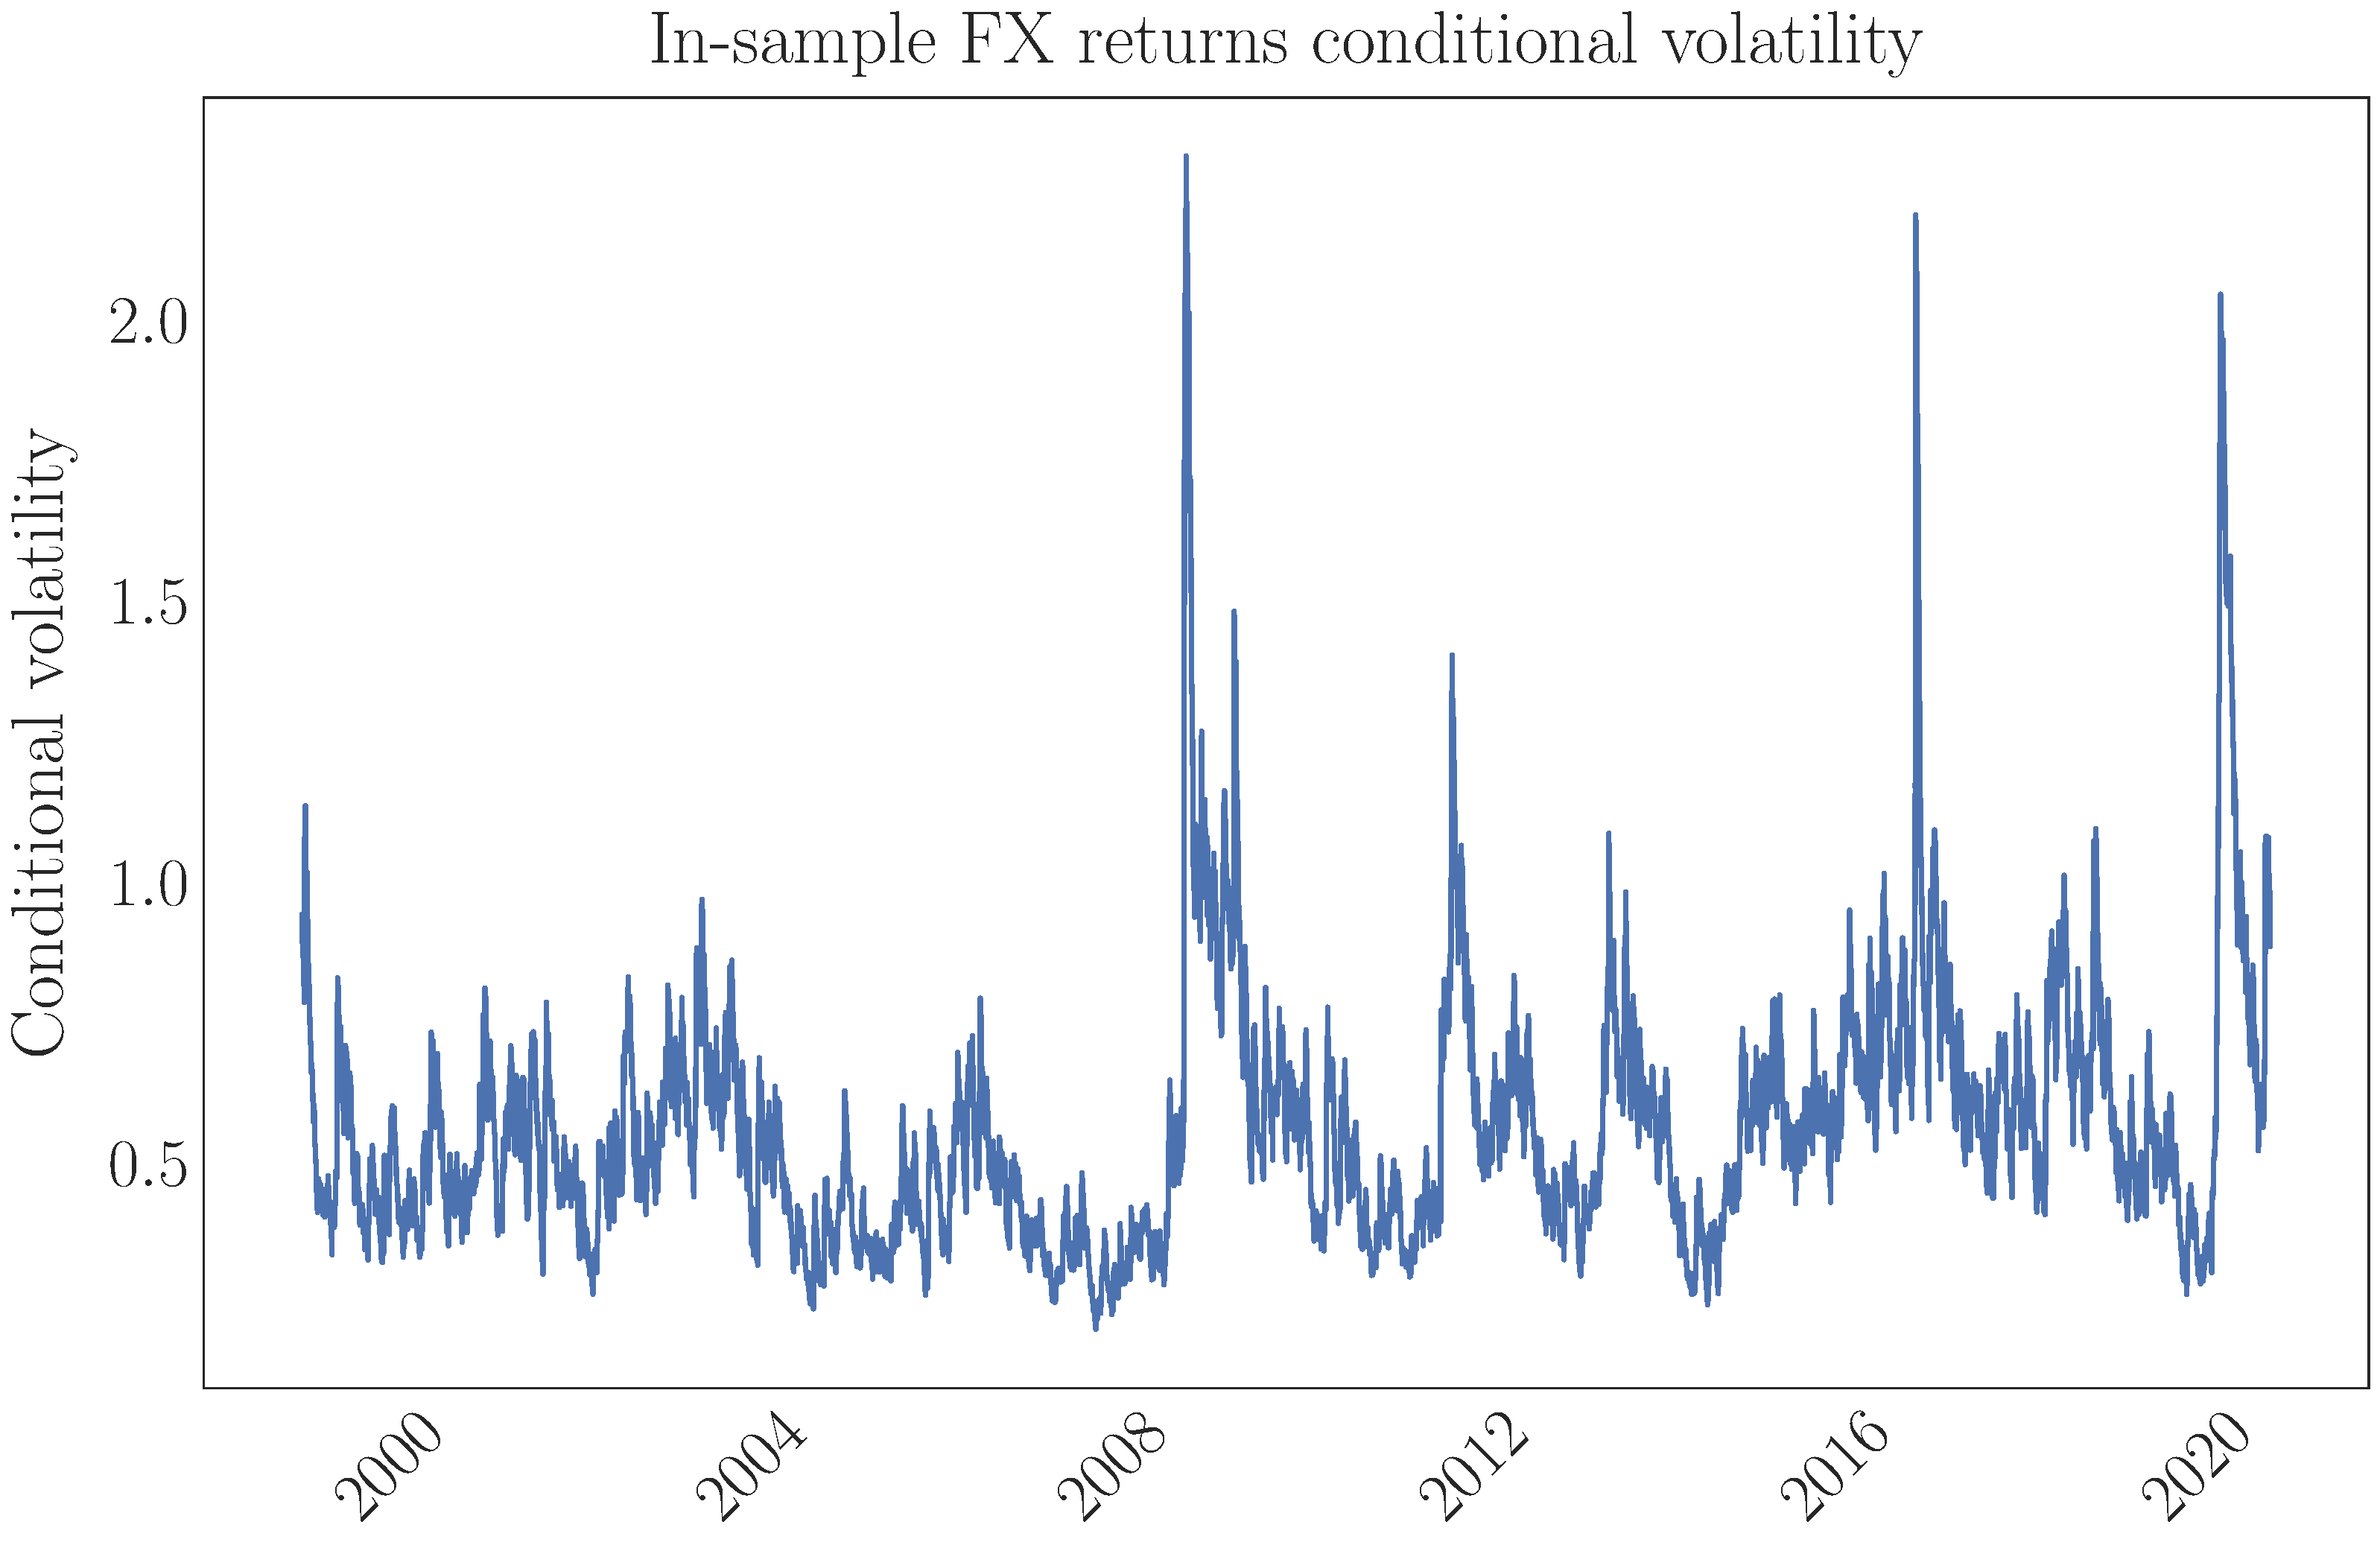
\includegraphics[width=\paperwidth]{conditional_vol_plot.pdf}}
\end{frame}

%% ---------------------------------------------------------------------------
%% Forecasting
%% ---------------------------------------------------------------------------
\section{Forecasting}

\begin{frame}
  \frametitle{Forecasting}

  \begin{largeitemize}
      \item Real-time forecasting based on market conditions
    \item Estimate the GARCH and derive the forecasted drift and volatility
    \item Infer the \textbf{full-fledged conditional distribution} of FX log returns for any point
      in time
    \item Assess model accuracy via (i) in-sample metrics and (ii) out of
      sample performance (probability integral transform test)
    \item The probability integral transform test assess on whether the random
      variable defined as $PIT(R) \equiv F_{R}R$ is uniformally distributed
      $F_{R}R \sim U(0,1)$, where $R$ is the stochastic process of the FX log returns $r_t, \forall t \in
      [0, T]$
  \end{largeitemize}
  
\end{frame}


\begin{frame}
\makebox[\linewidth]{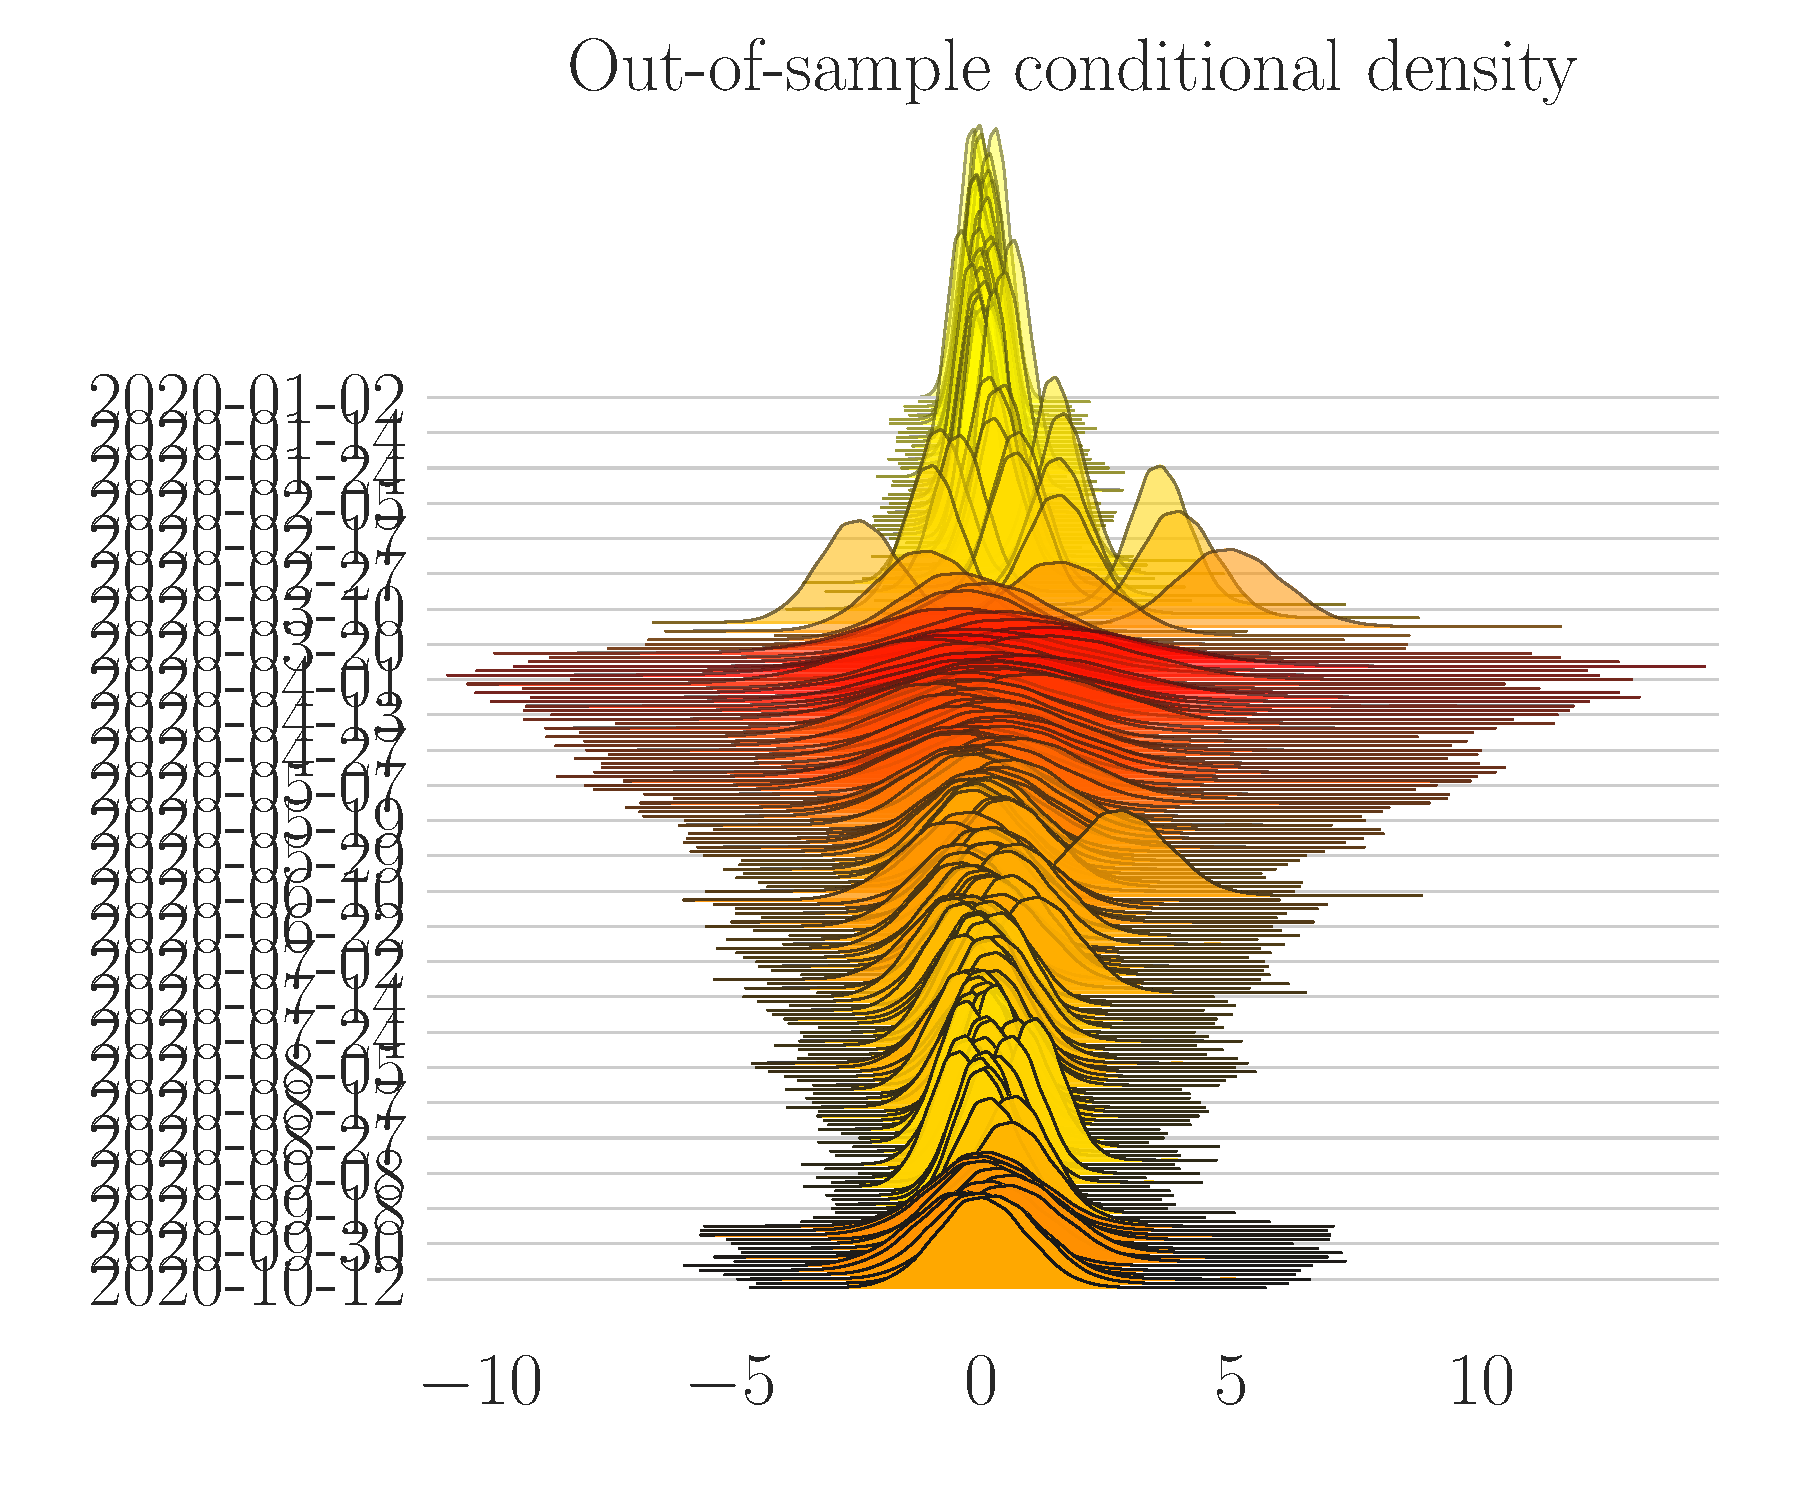
\includegraphics[width=\paperwidth, height=\paperheight]{joyplot.pdf}}
\end{frame}

\begin{frame}
 \frametitle{Fan Chart}
\makebox[\linewidth]{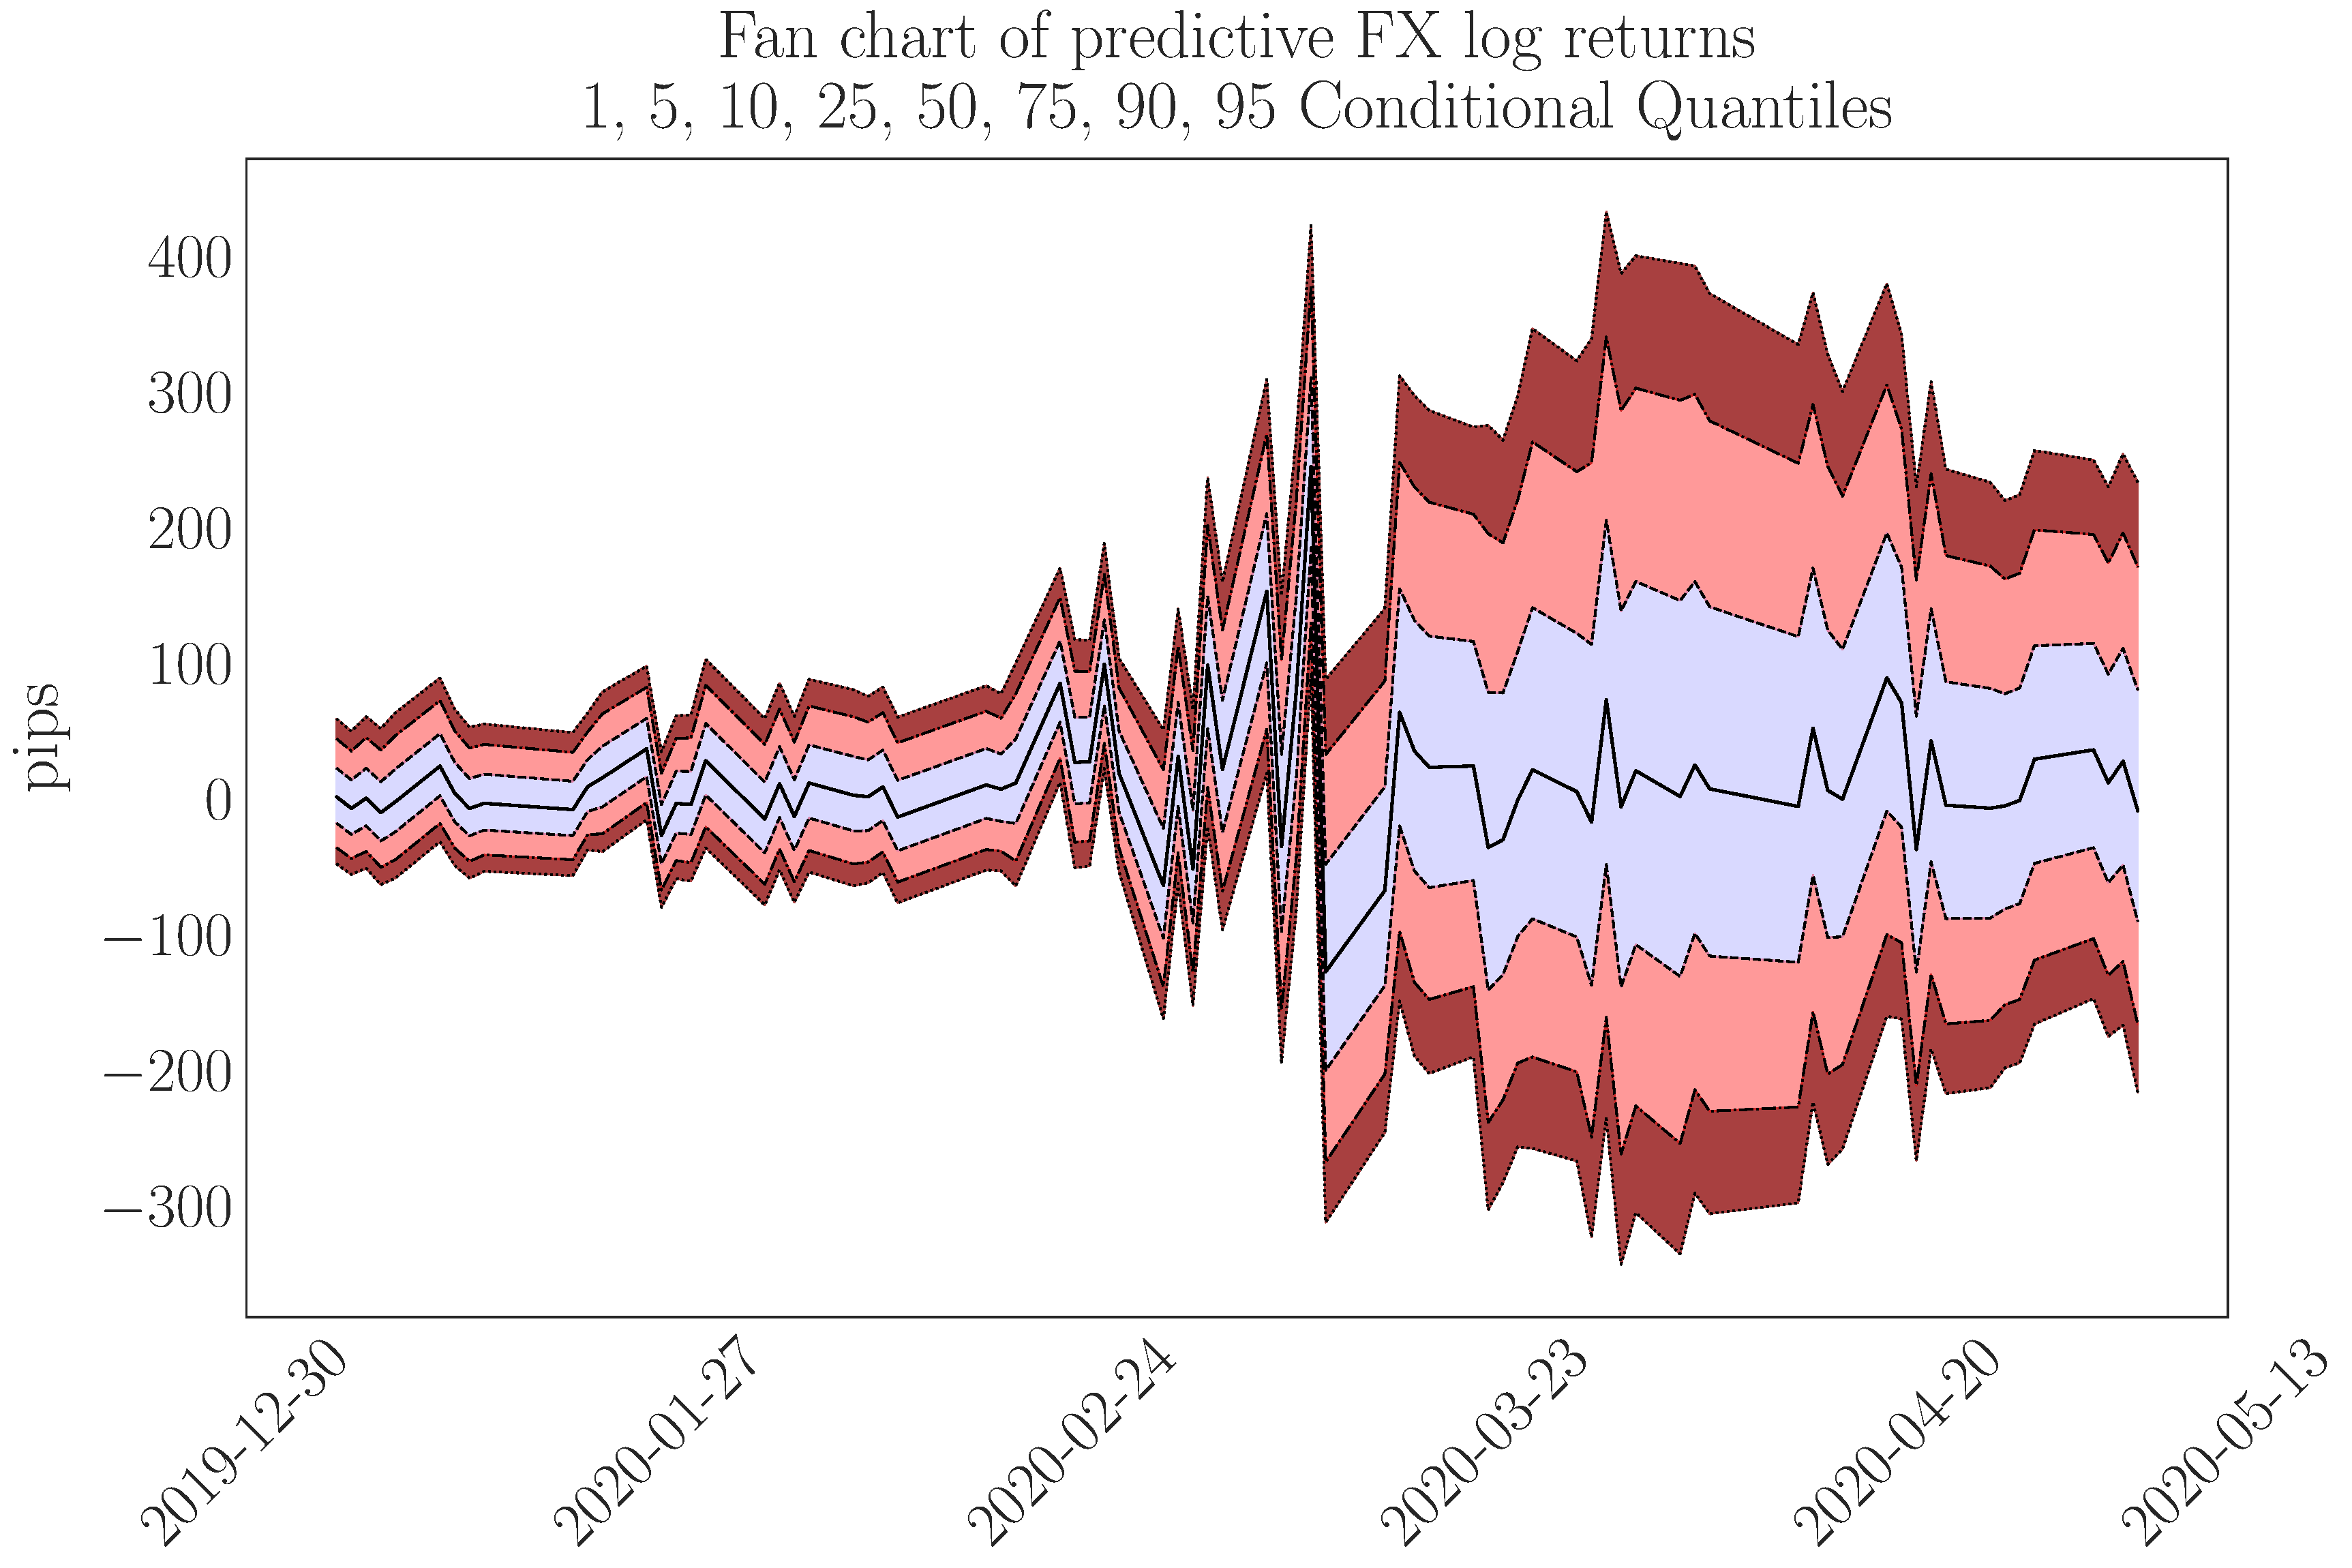
\includegraphics[width=0.95\paperwidth]{fanchart.pdf}}
\end{frame}

\begin{frame}
  \frametitle{VaR FXI Rule}
    \makebox[\linewidth]{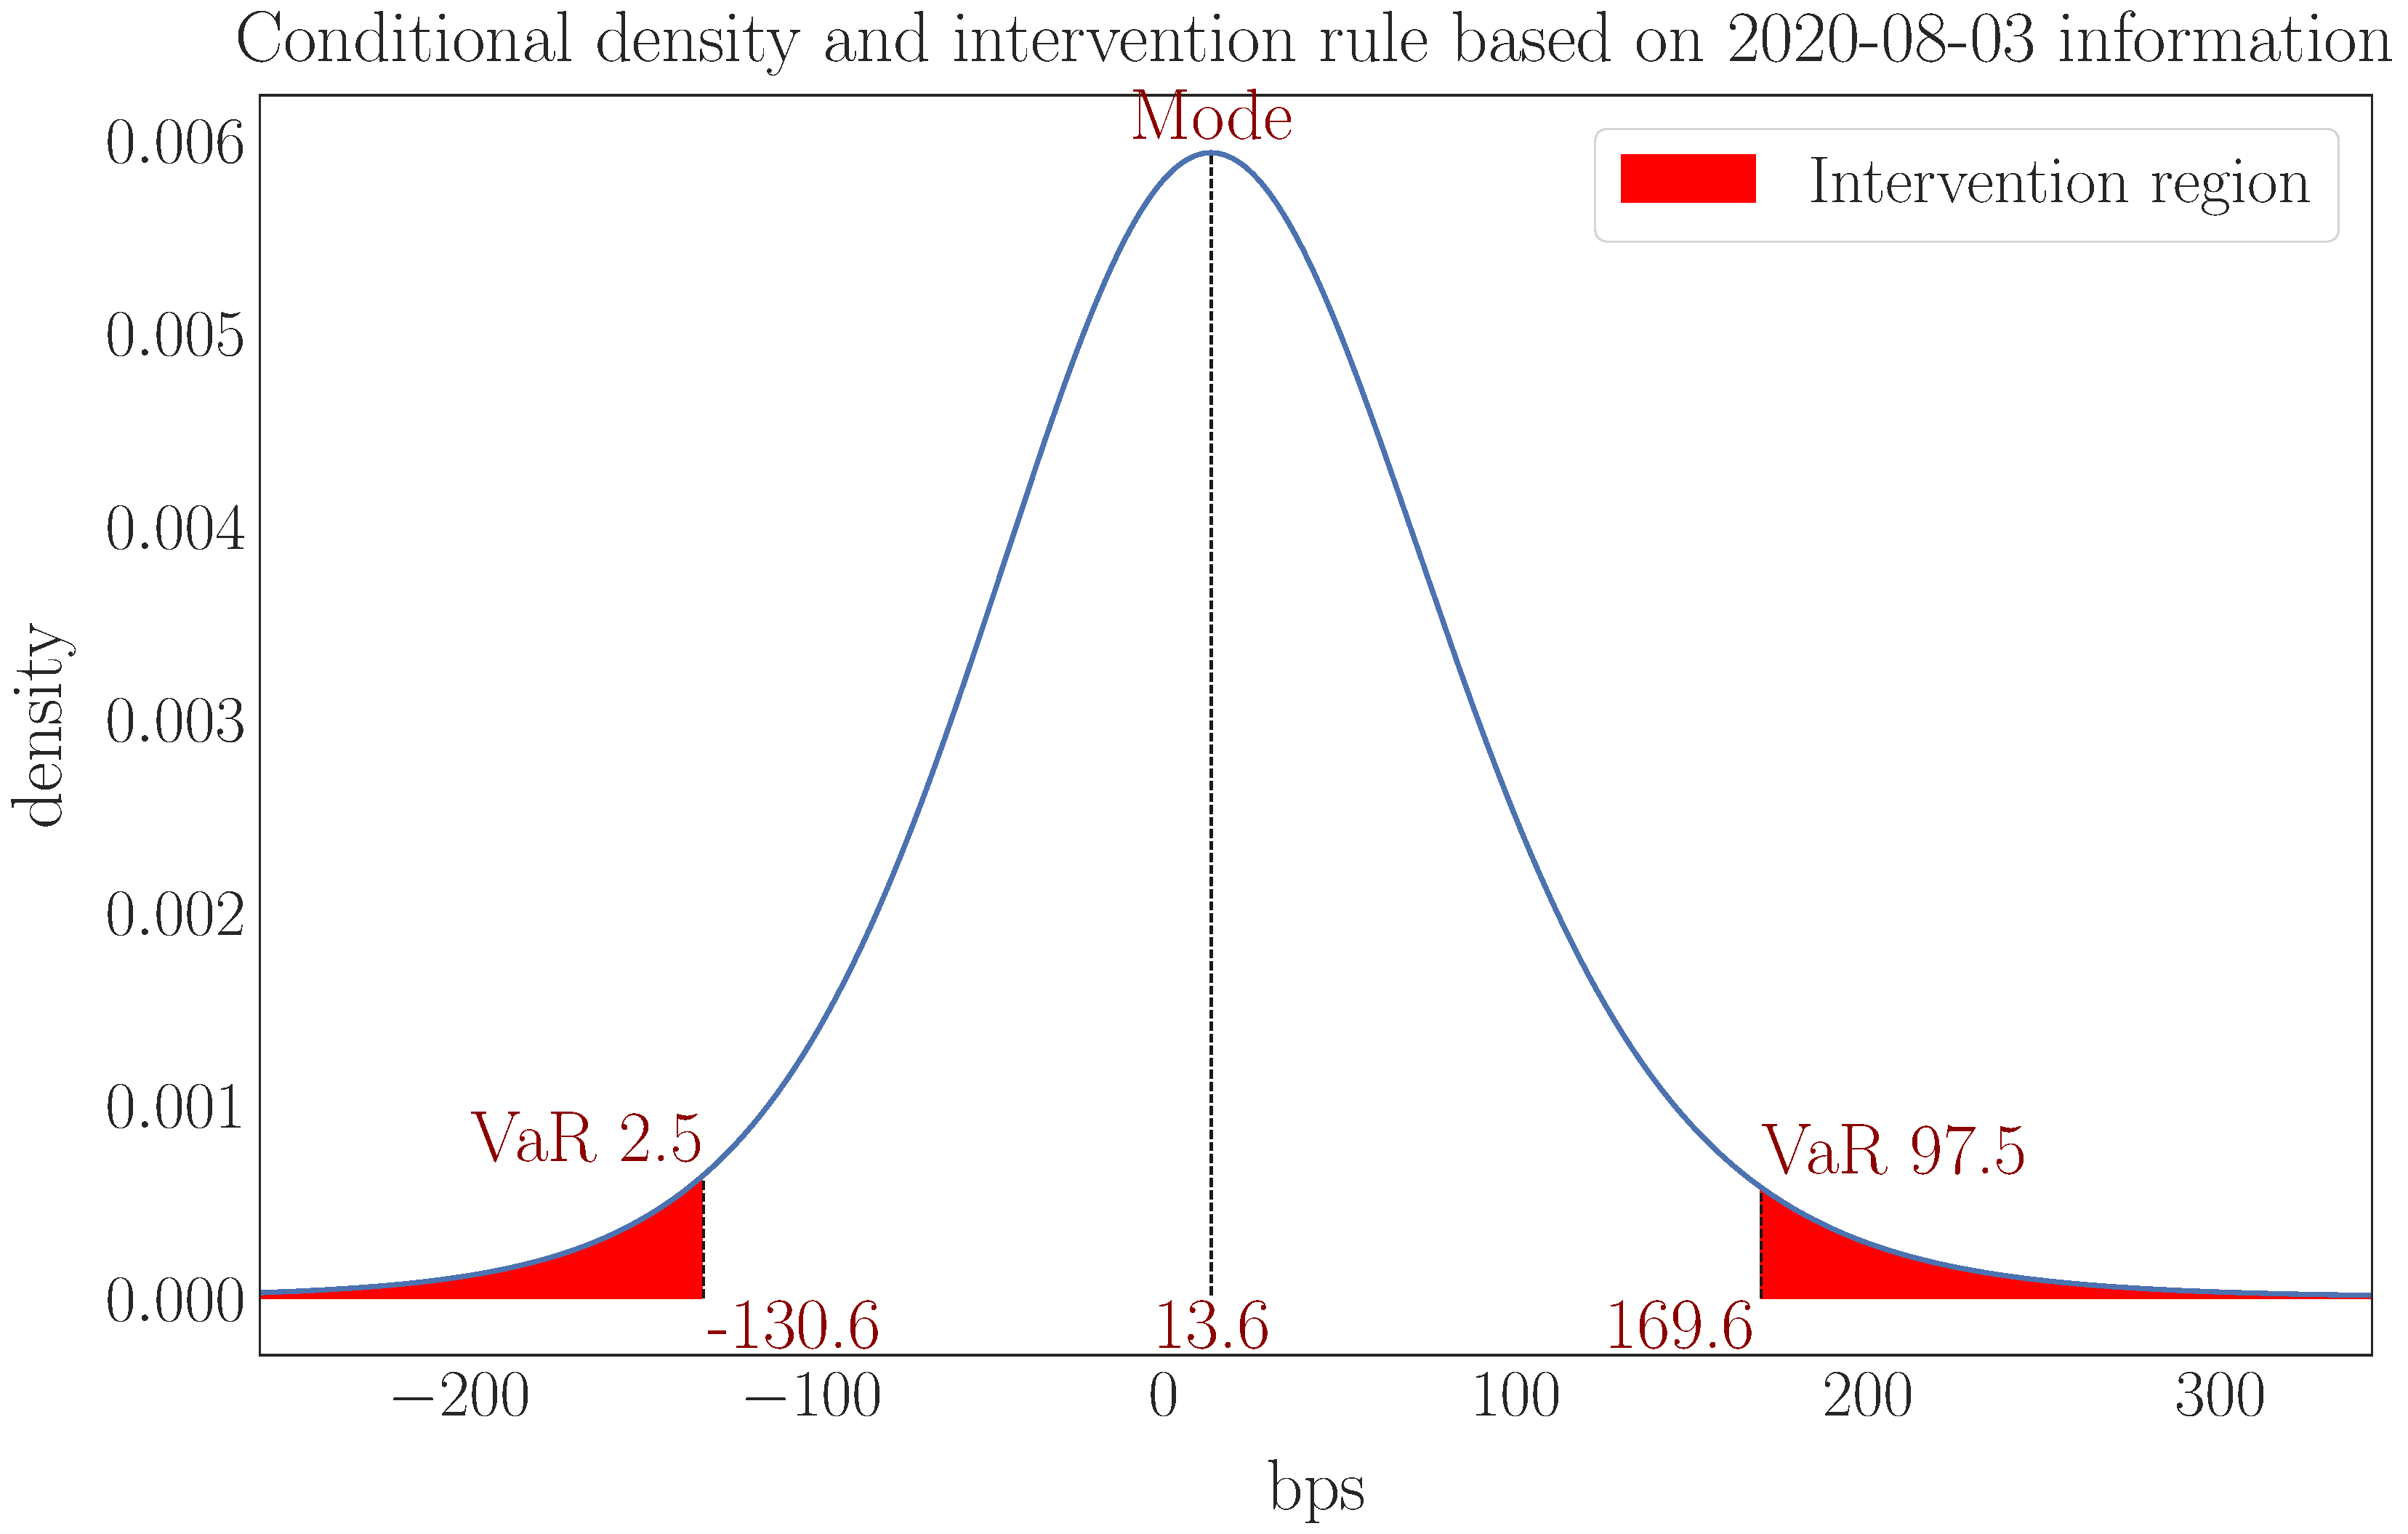
\includegraphics[width=\paperwidth]{var_rule.pdf}}
\end{frame}

\begin{frame}
  \frametitle{Conditional Cumulative Distribution Function}
    \makebox[\linewidth]{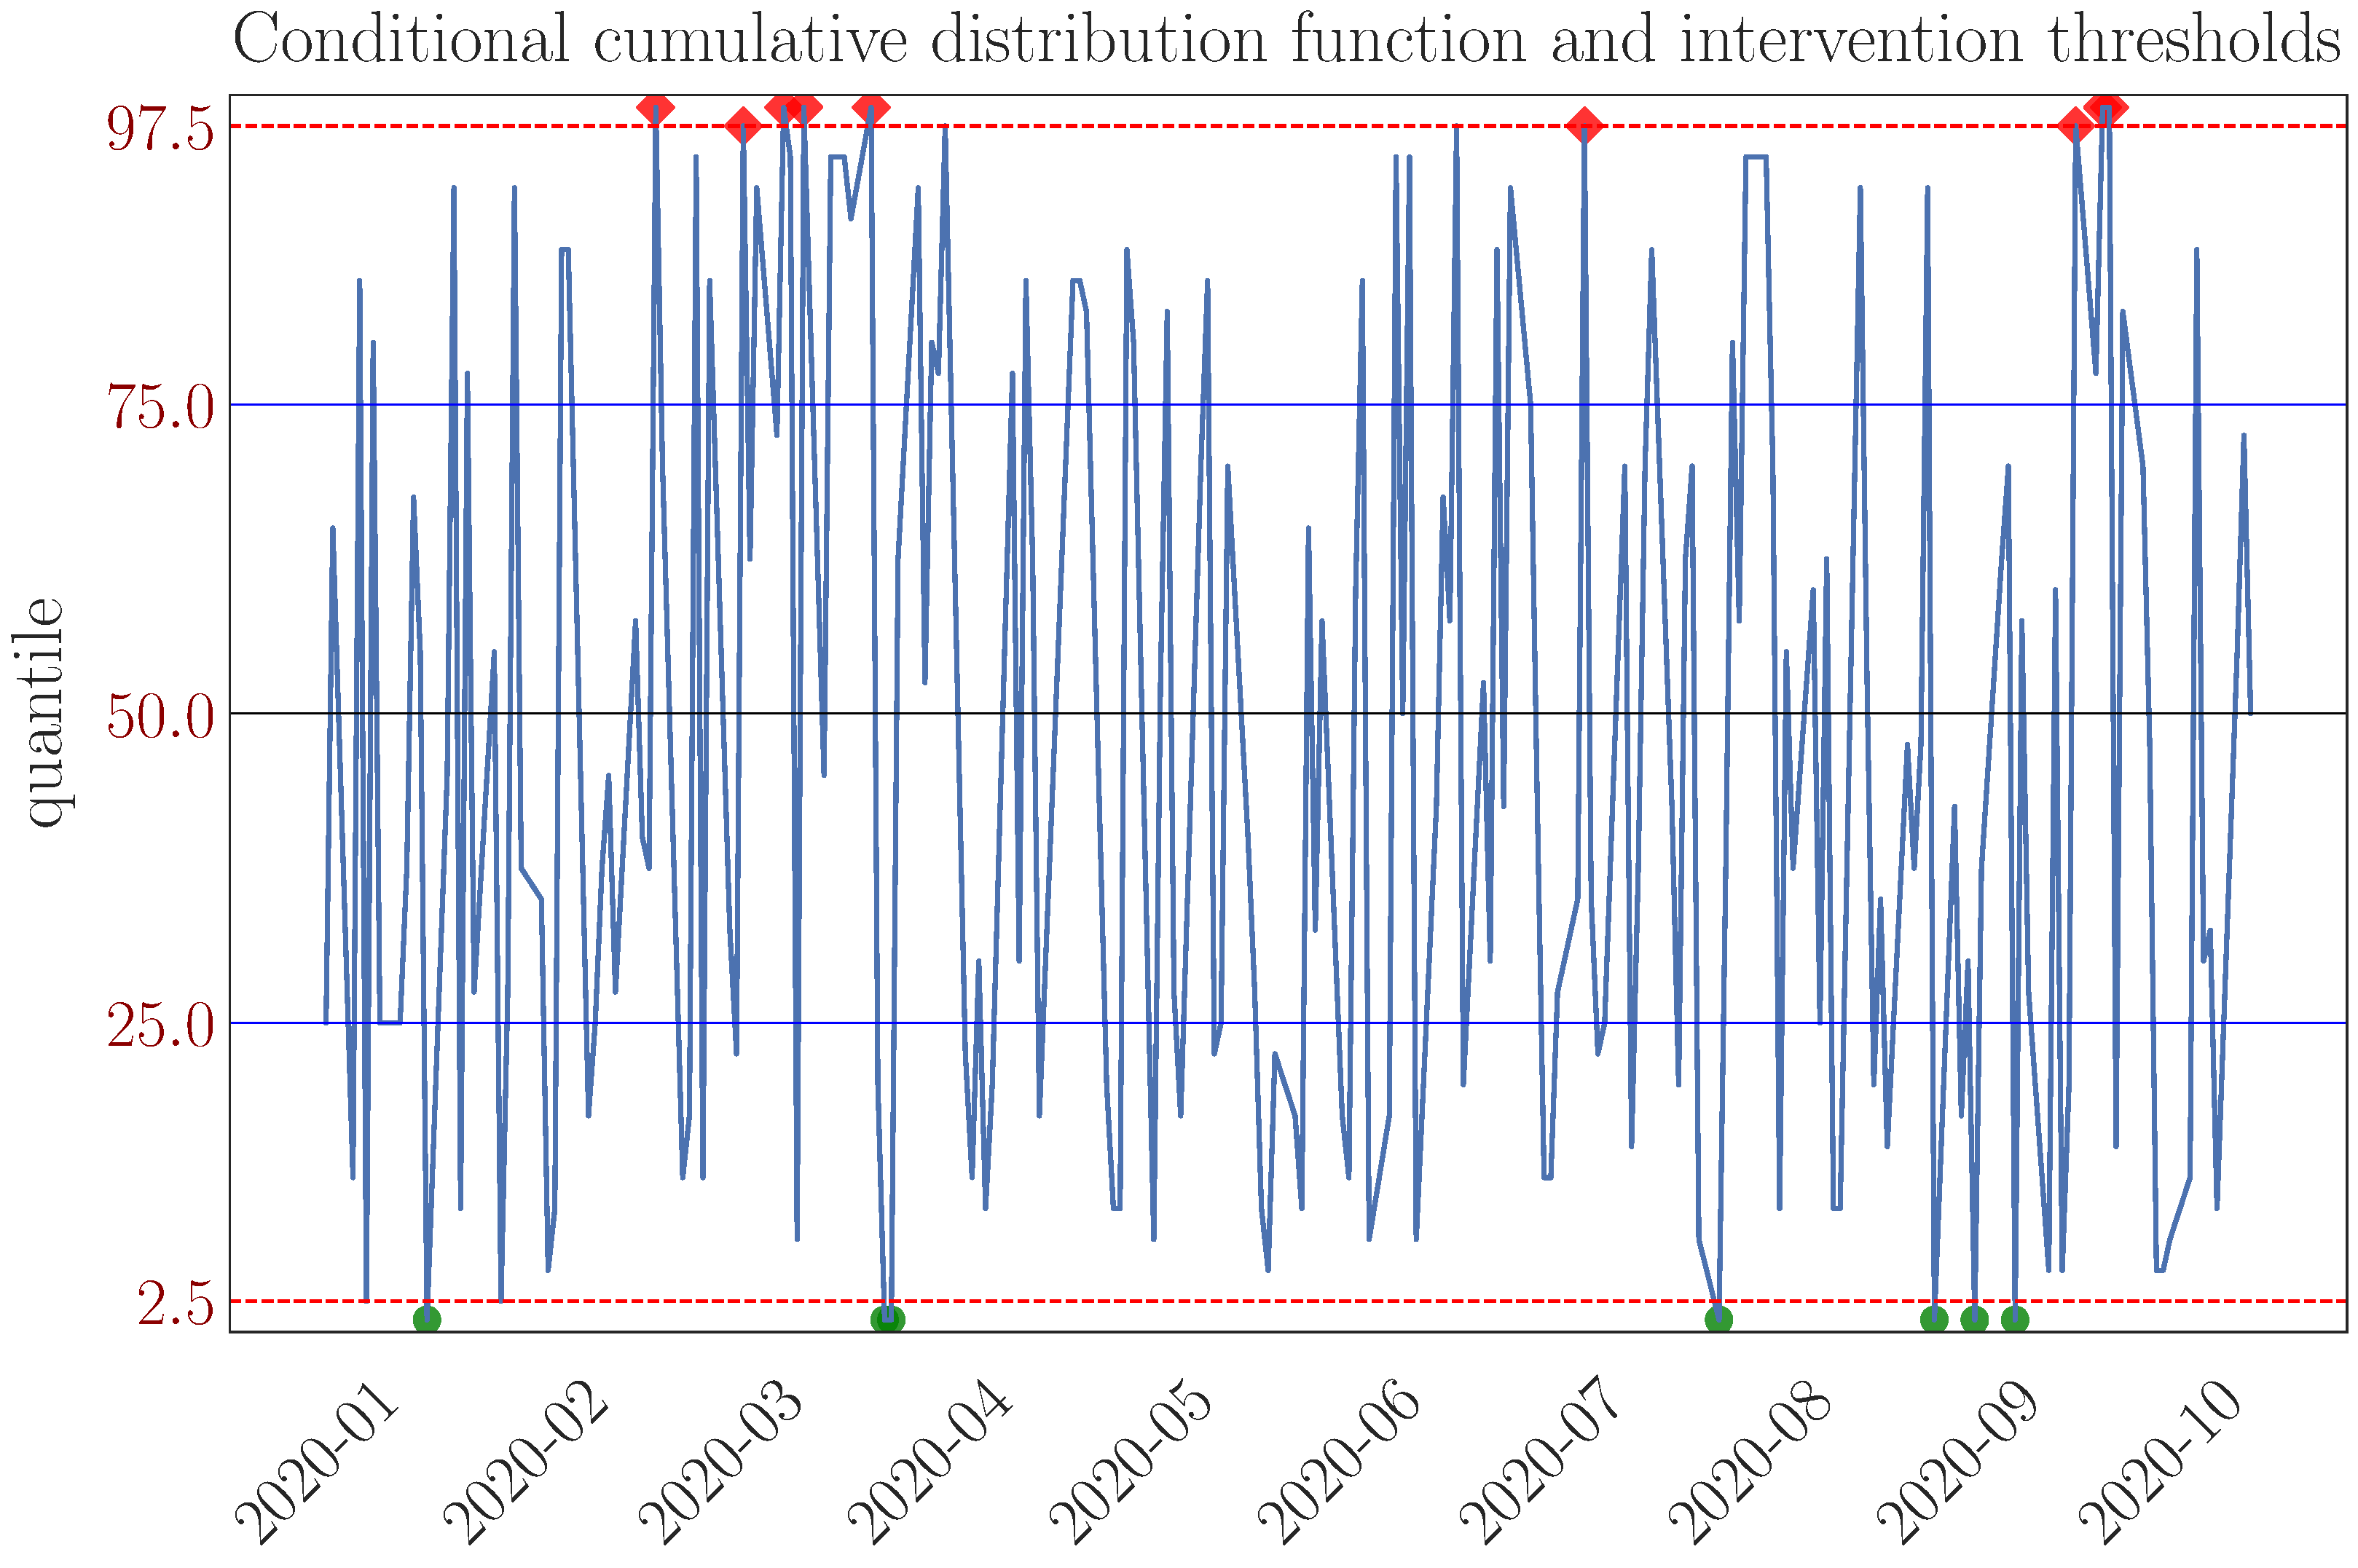
\includegraphics[width=\paperwidth]{conditional_cdf.pdf}}
\end{frame}

\begin{frame}
  \frametitle{Conditional Exceedance}
    \makebox[\linewidth]{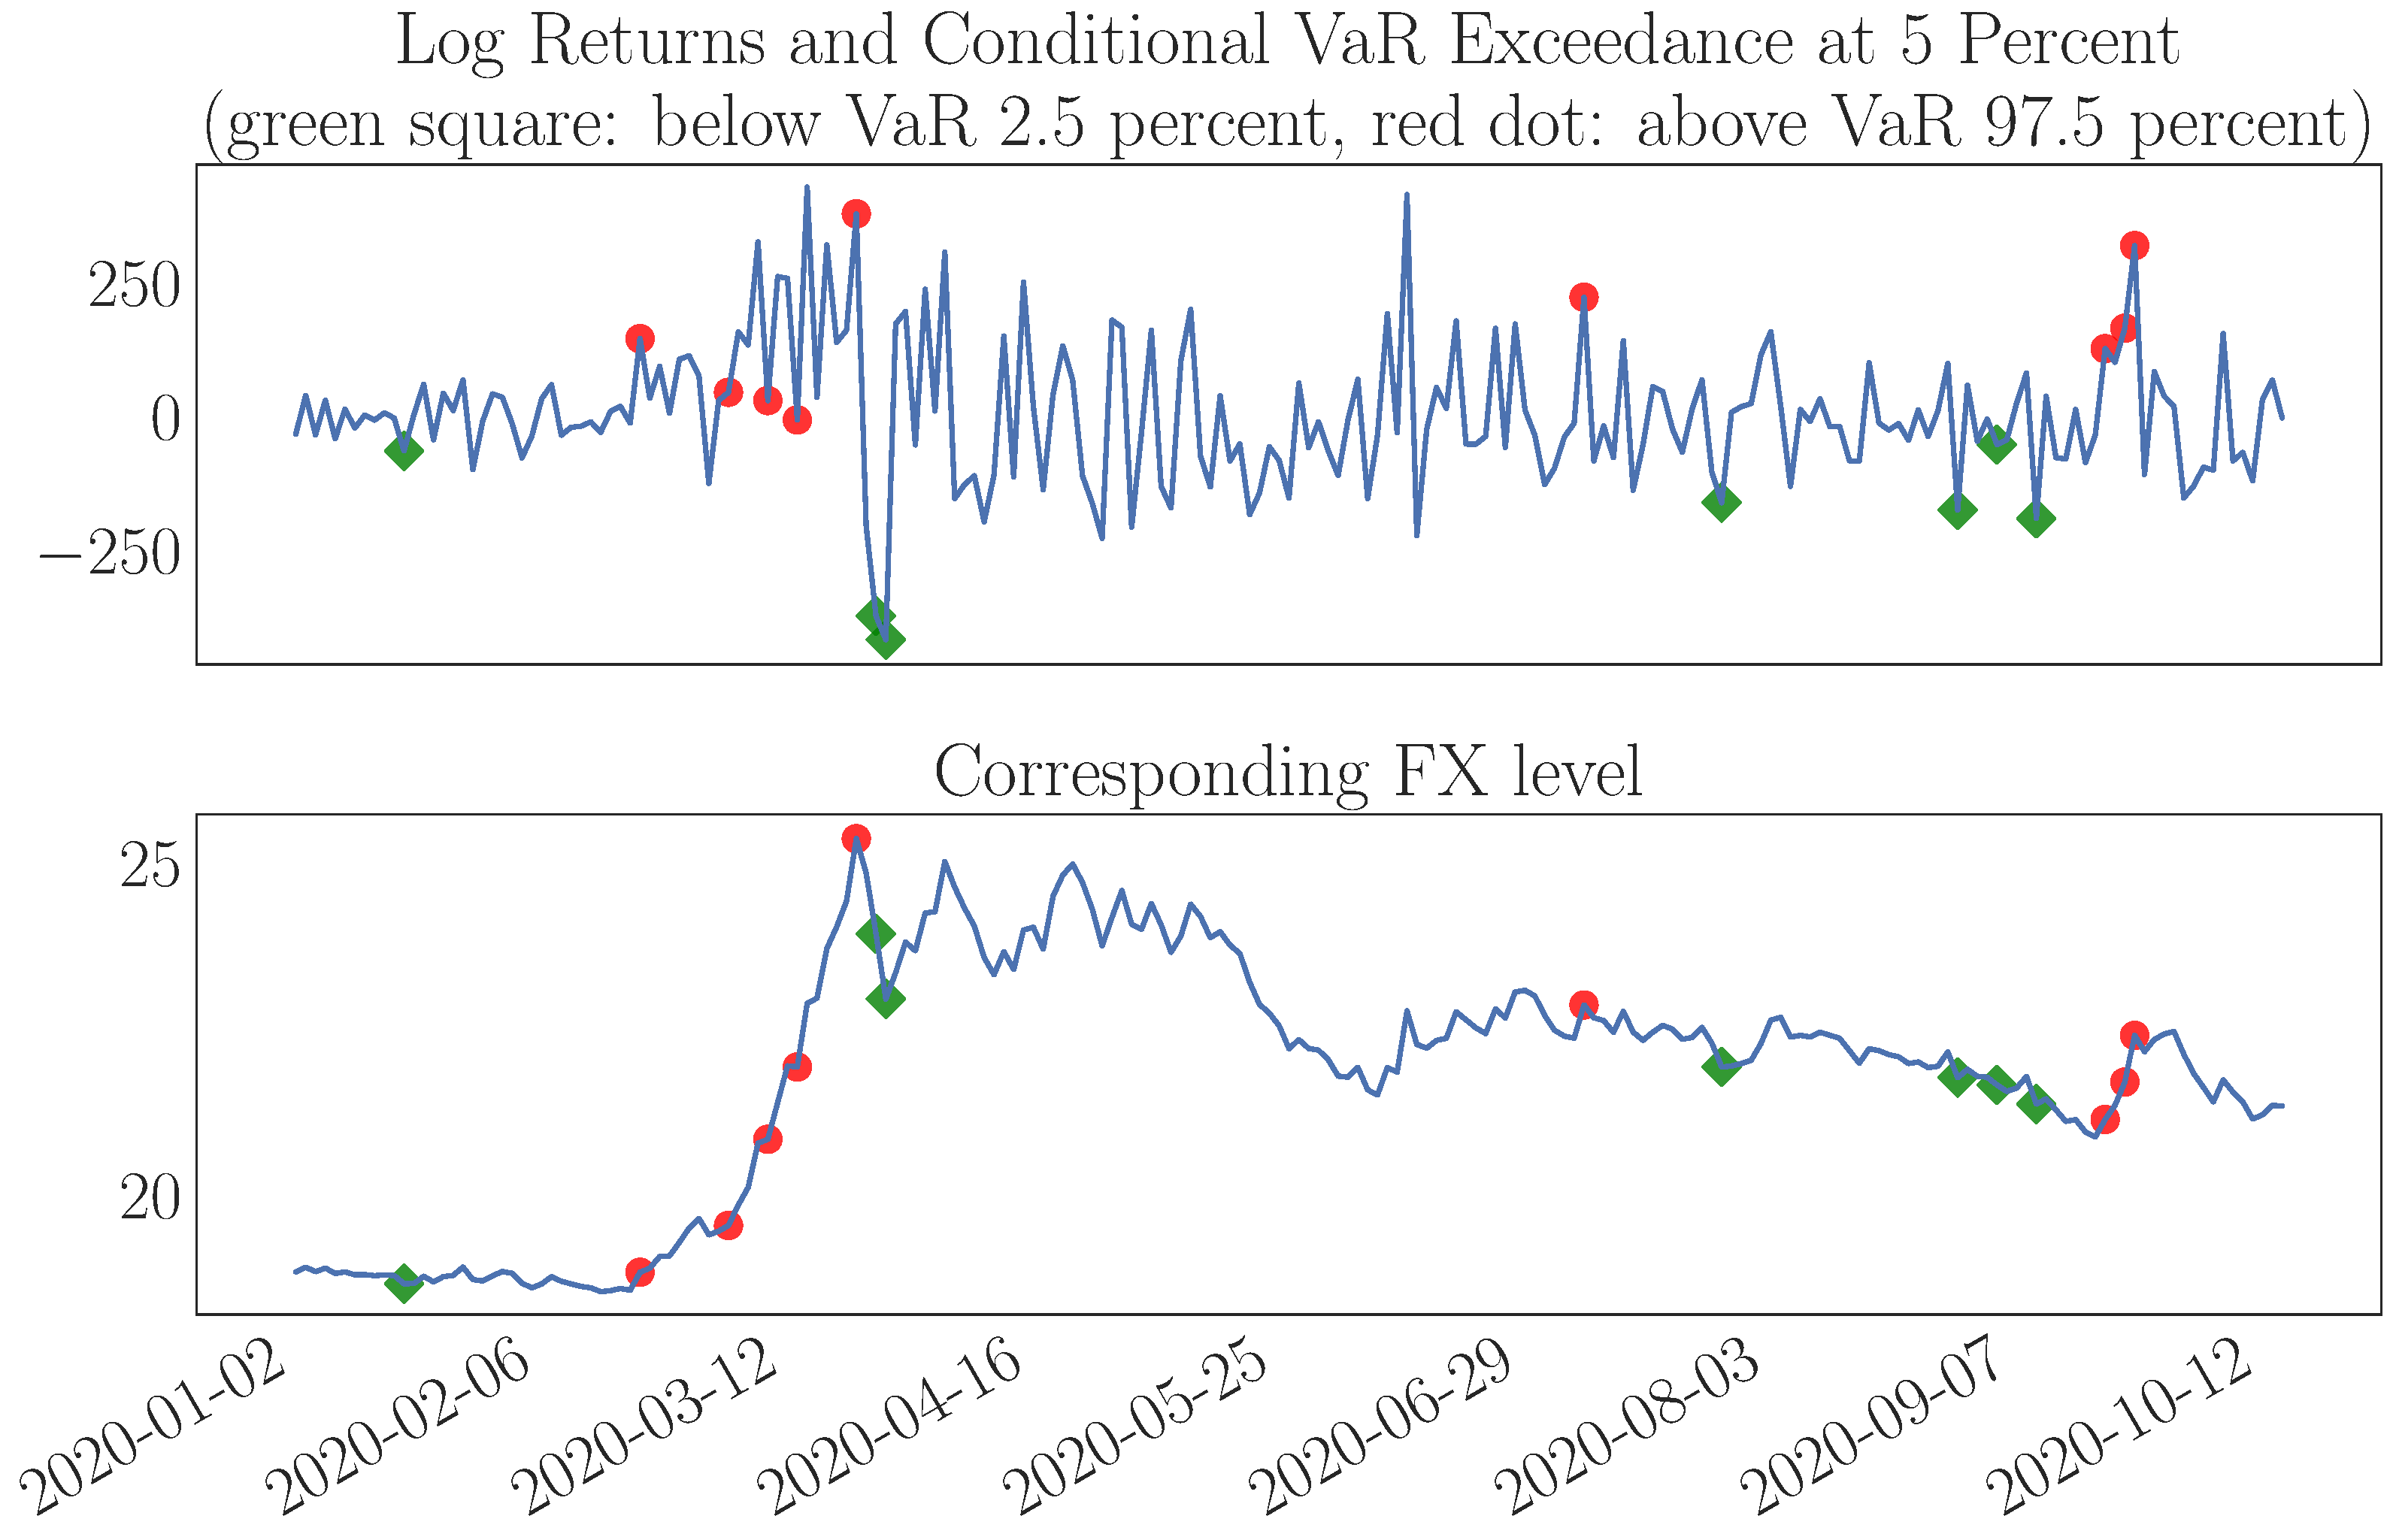
\includegraphics[width=\paperwidth]{conditional_exceedance.pdf}}
\end{frame}

\begin{frame}
  \frametitle{Density Evaluation}
    \makebox[\linewidth]{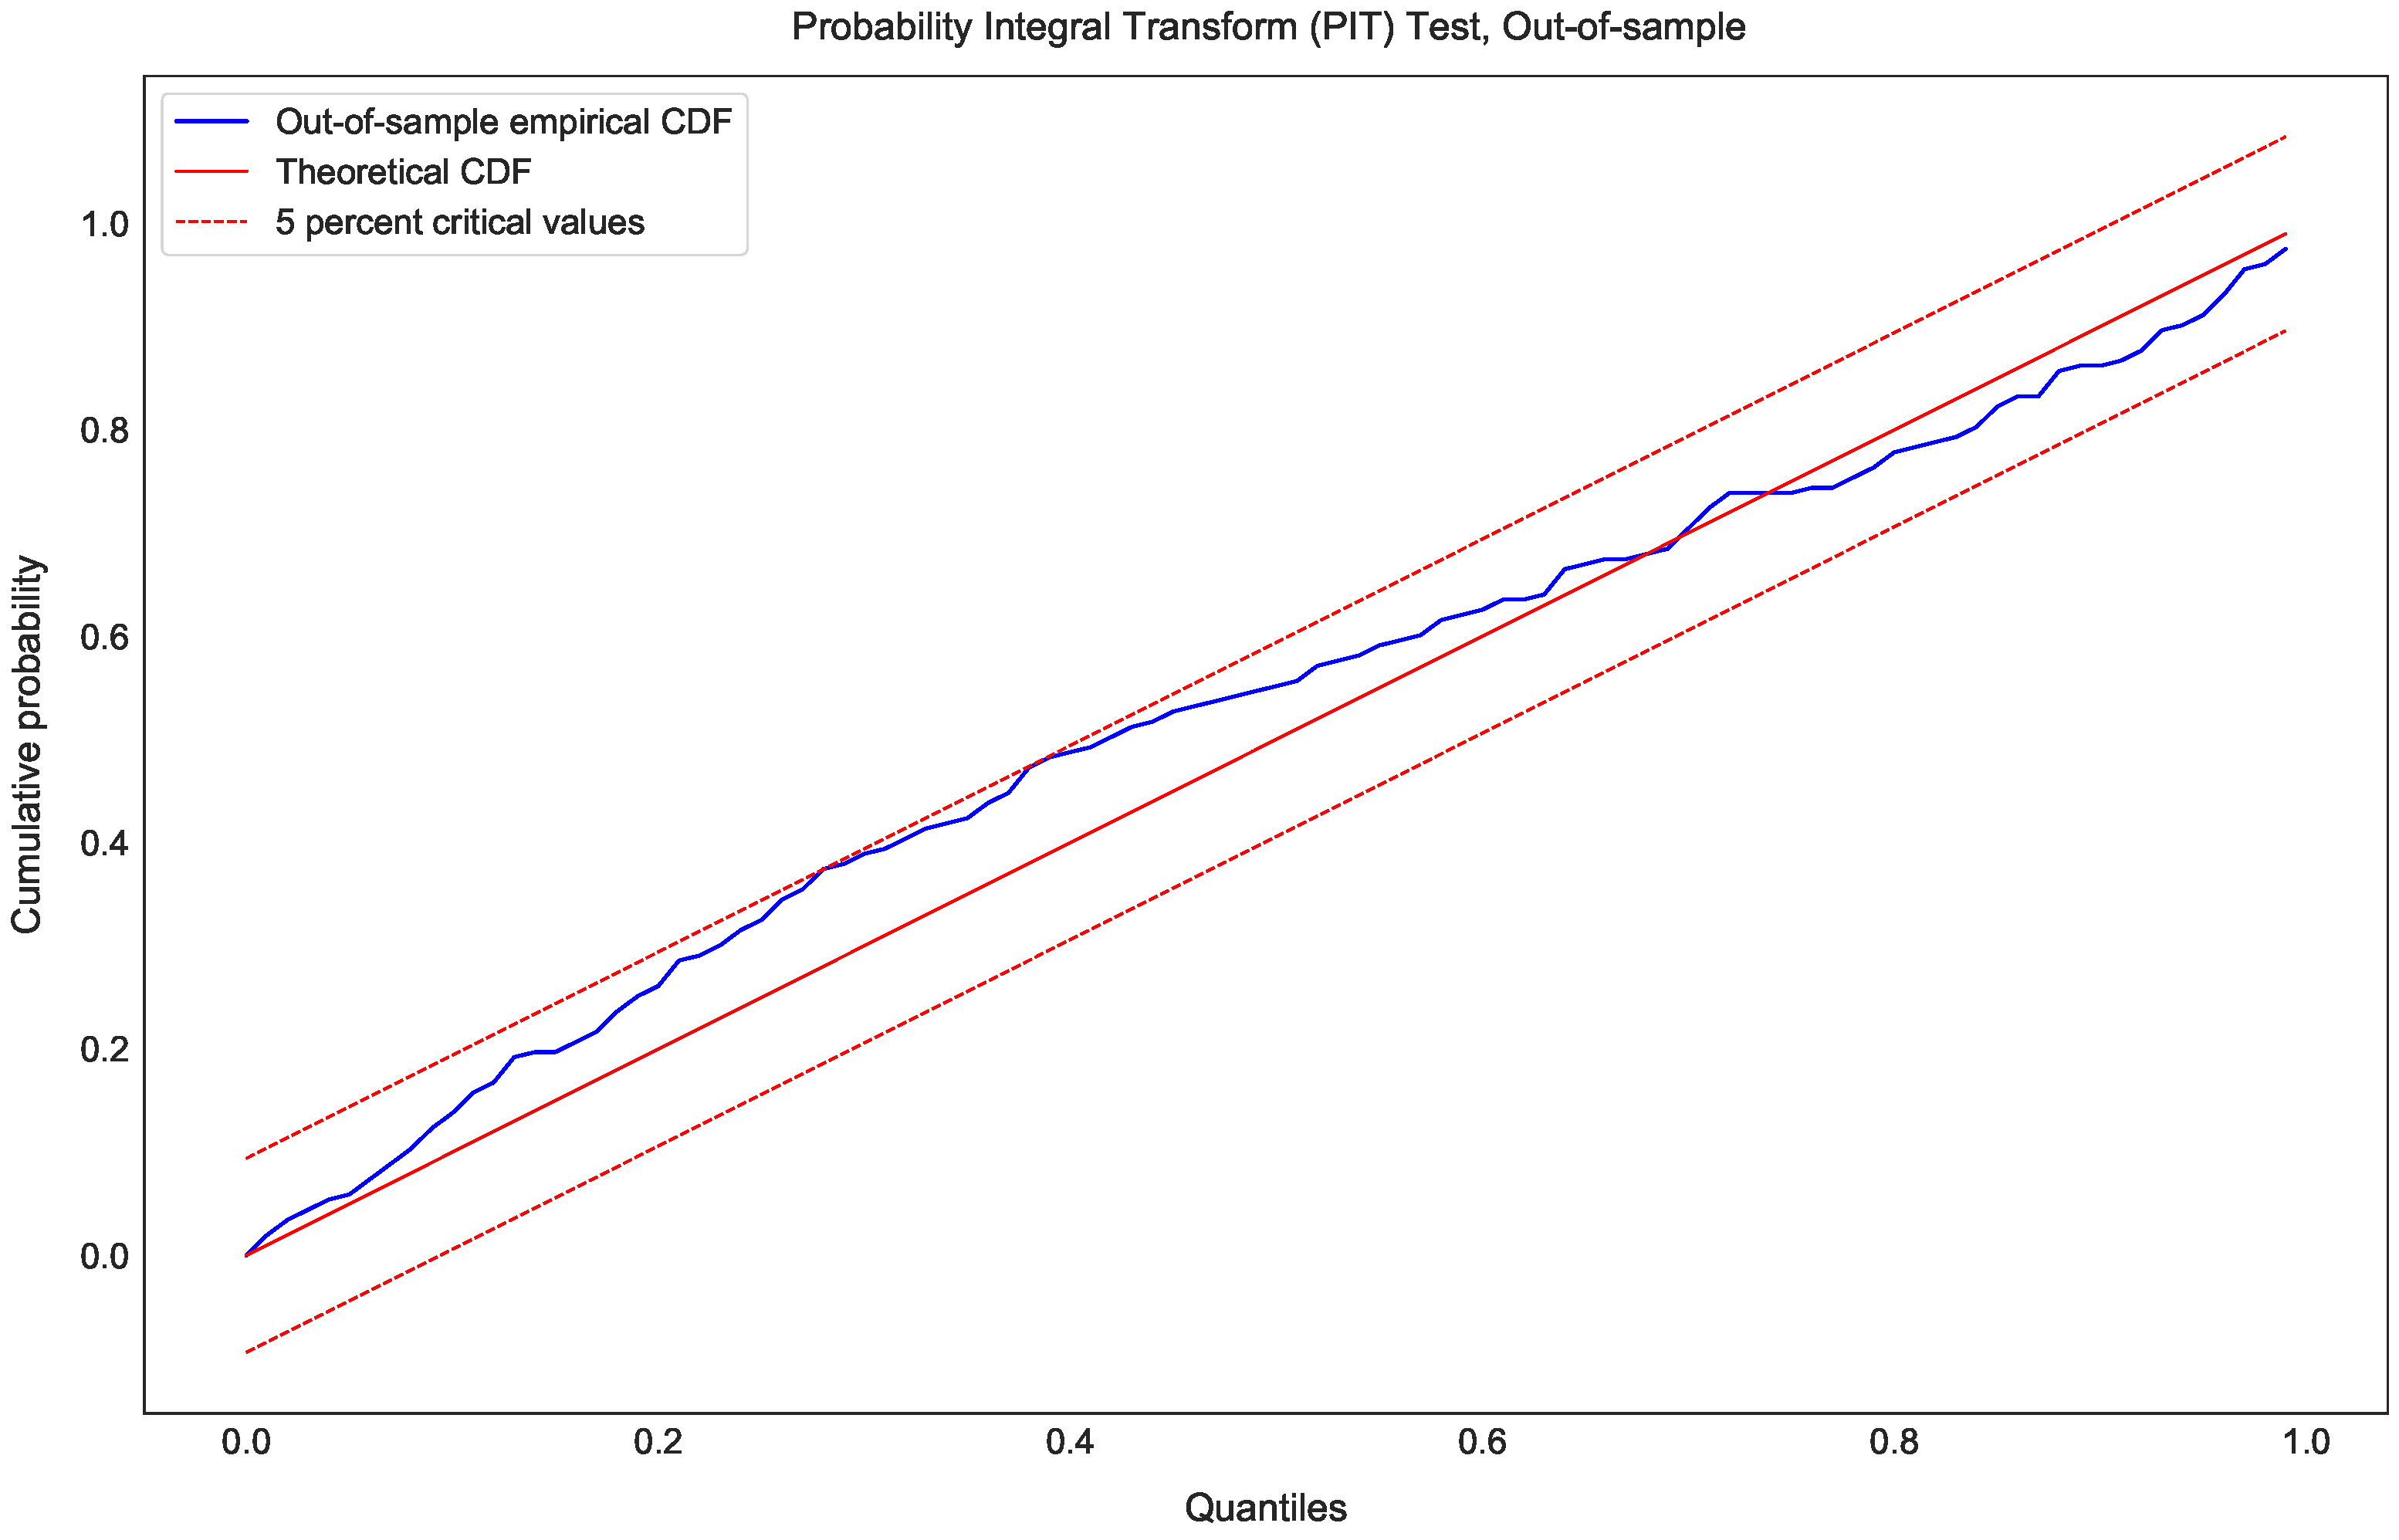
\includegraphics[width=\paperwidth]{pitchart.pdf}}
\end{frame}


%% ---------------------------------------------------------------------------
%% Benchmarking
%% ---------------------------------------------------------------------------
\section{Benchmarking}

\begin{frame}
  \frametitle{Bank of Mexico FX Interventions Setup}  
  \begin{largeitemize}
    \item The Banco Mexico (BM) implemented both discretionary and
      fixed-volatility FXI and intervened via transparent FX auctions
    \item Difference between rule and discretion was the reservation rate applied to the auction:
      \begin{itemize}
      \item \textbf{Rule-based setting}: BM operated an auction every day
        with a pre-announced reservation rate, \textbf{a minimum rate} for
        eligible bids
      \item \textbf{Discretionary setting}: the auction was organized at the BM's discretion without reservation rate
      \end{itemize}
  \item Often, no demand for the ruled-based auction as the market rate was below the reservation rate
  \item Use the conditional cumulative distribution function (CDF) as
    benchmark: what was the risk level when the central bank intervened?
  \end{largeitemize}
\end{frame}


\begin{frame}
  \frametitle{Rule-Based Benchmarking}
    \makebox[\linewidth]{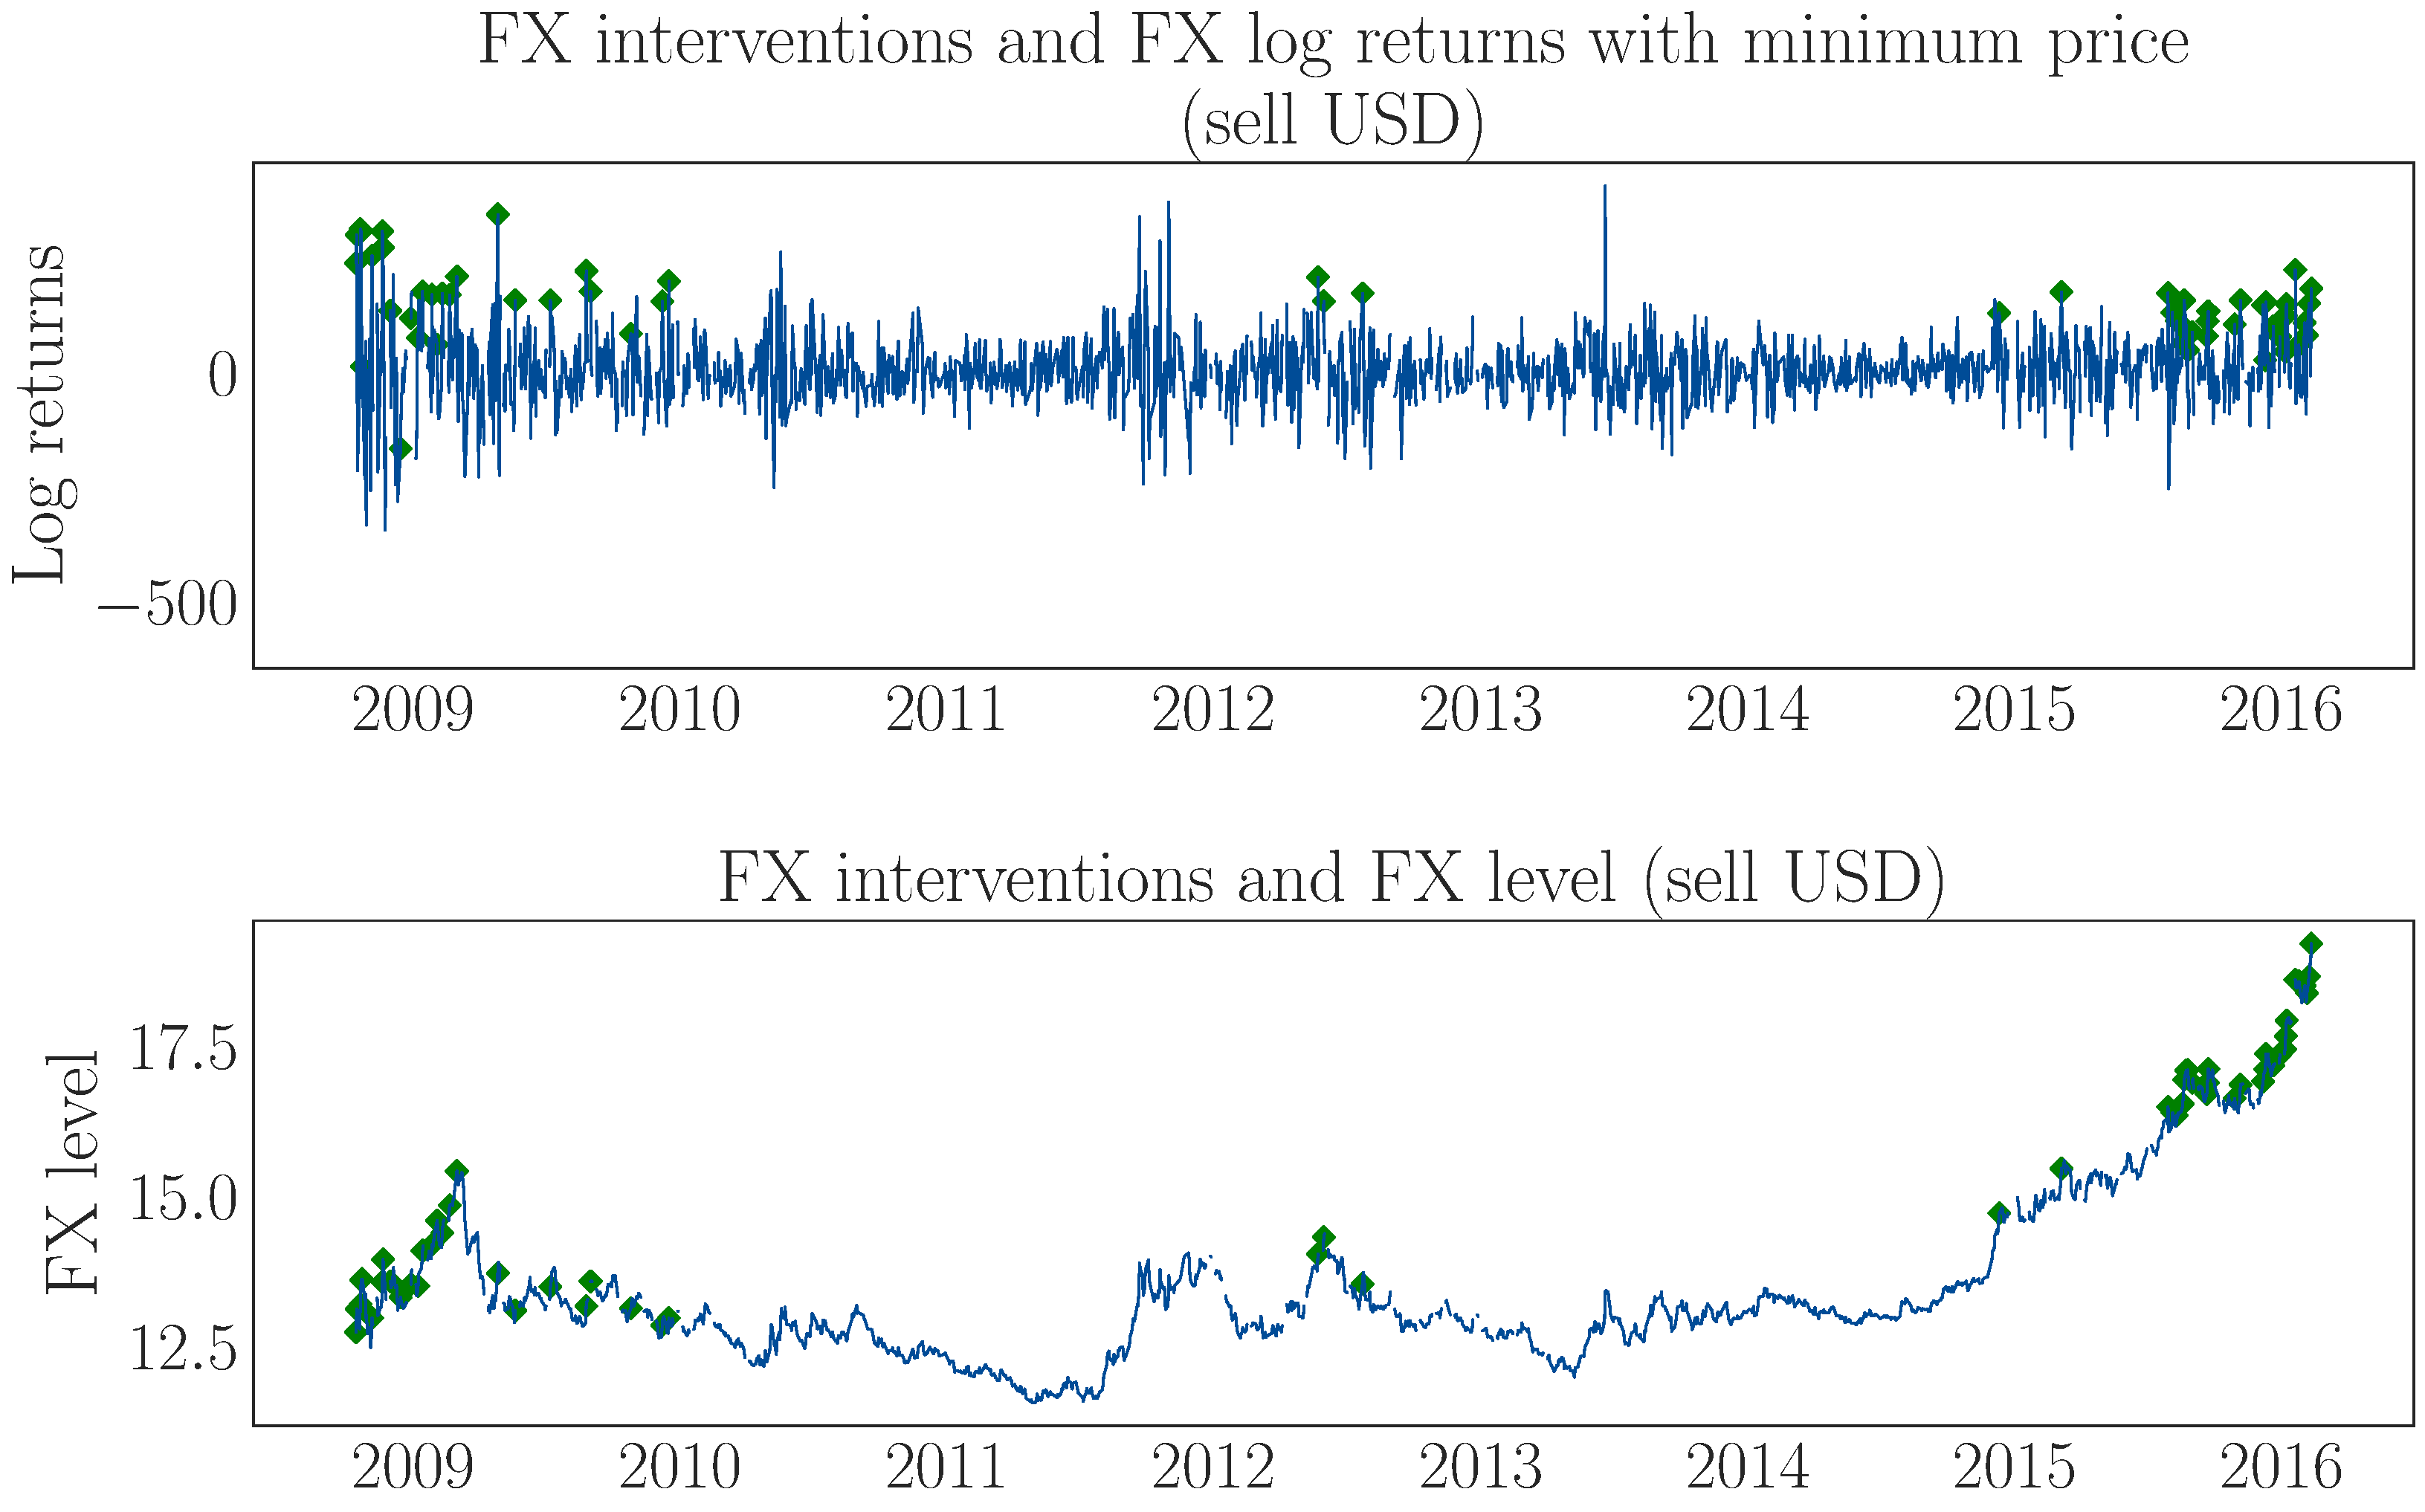
\includegraphics[width=\paperwidth]{benchmark_minprice.pdf}}
\end{frame}


\begin{frame}
  \frametitle{Rule-Based Benchmarking: Risk-Level}
    \makebox[\linewidth]{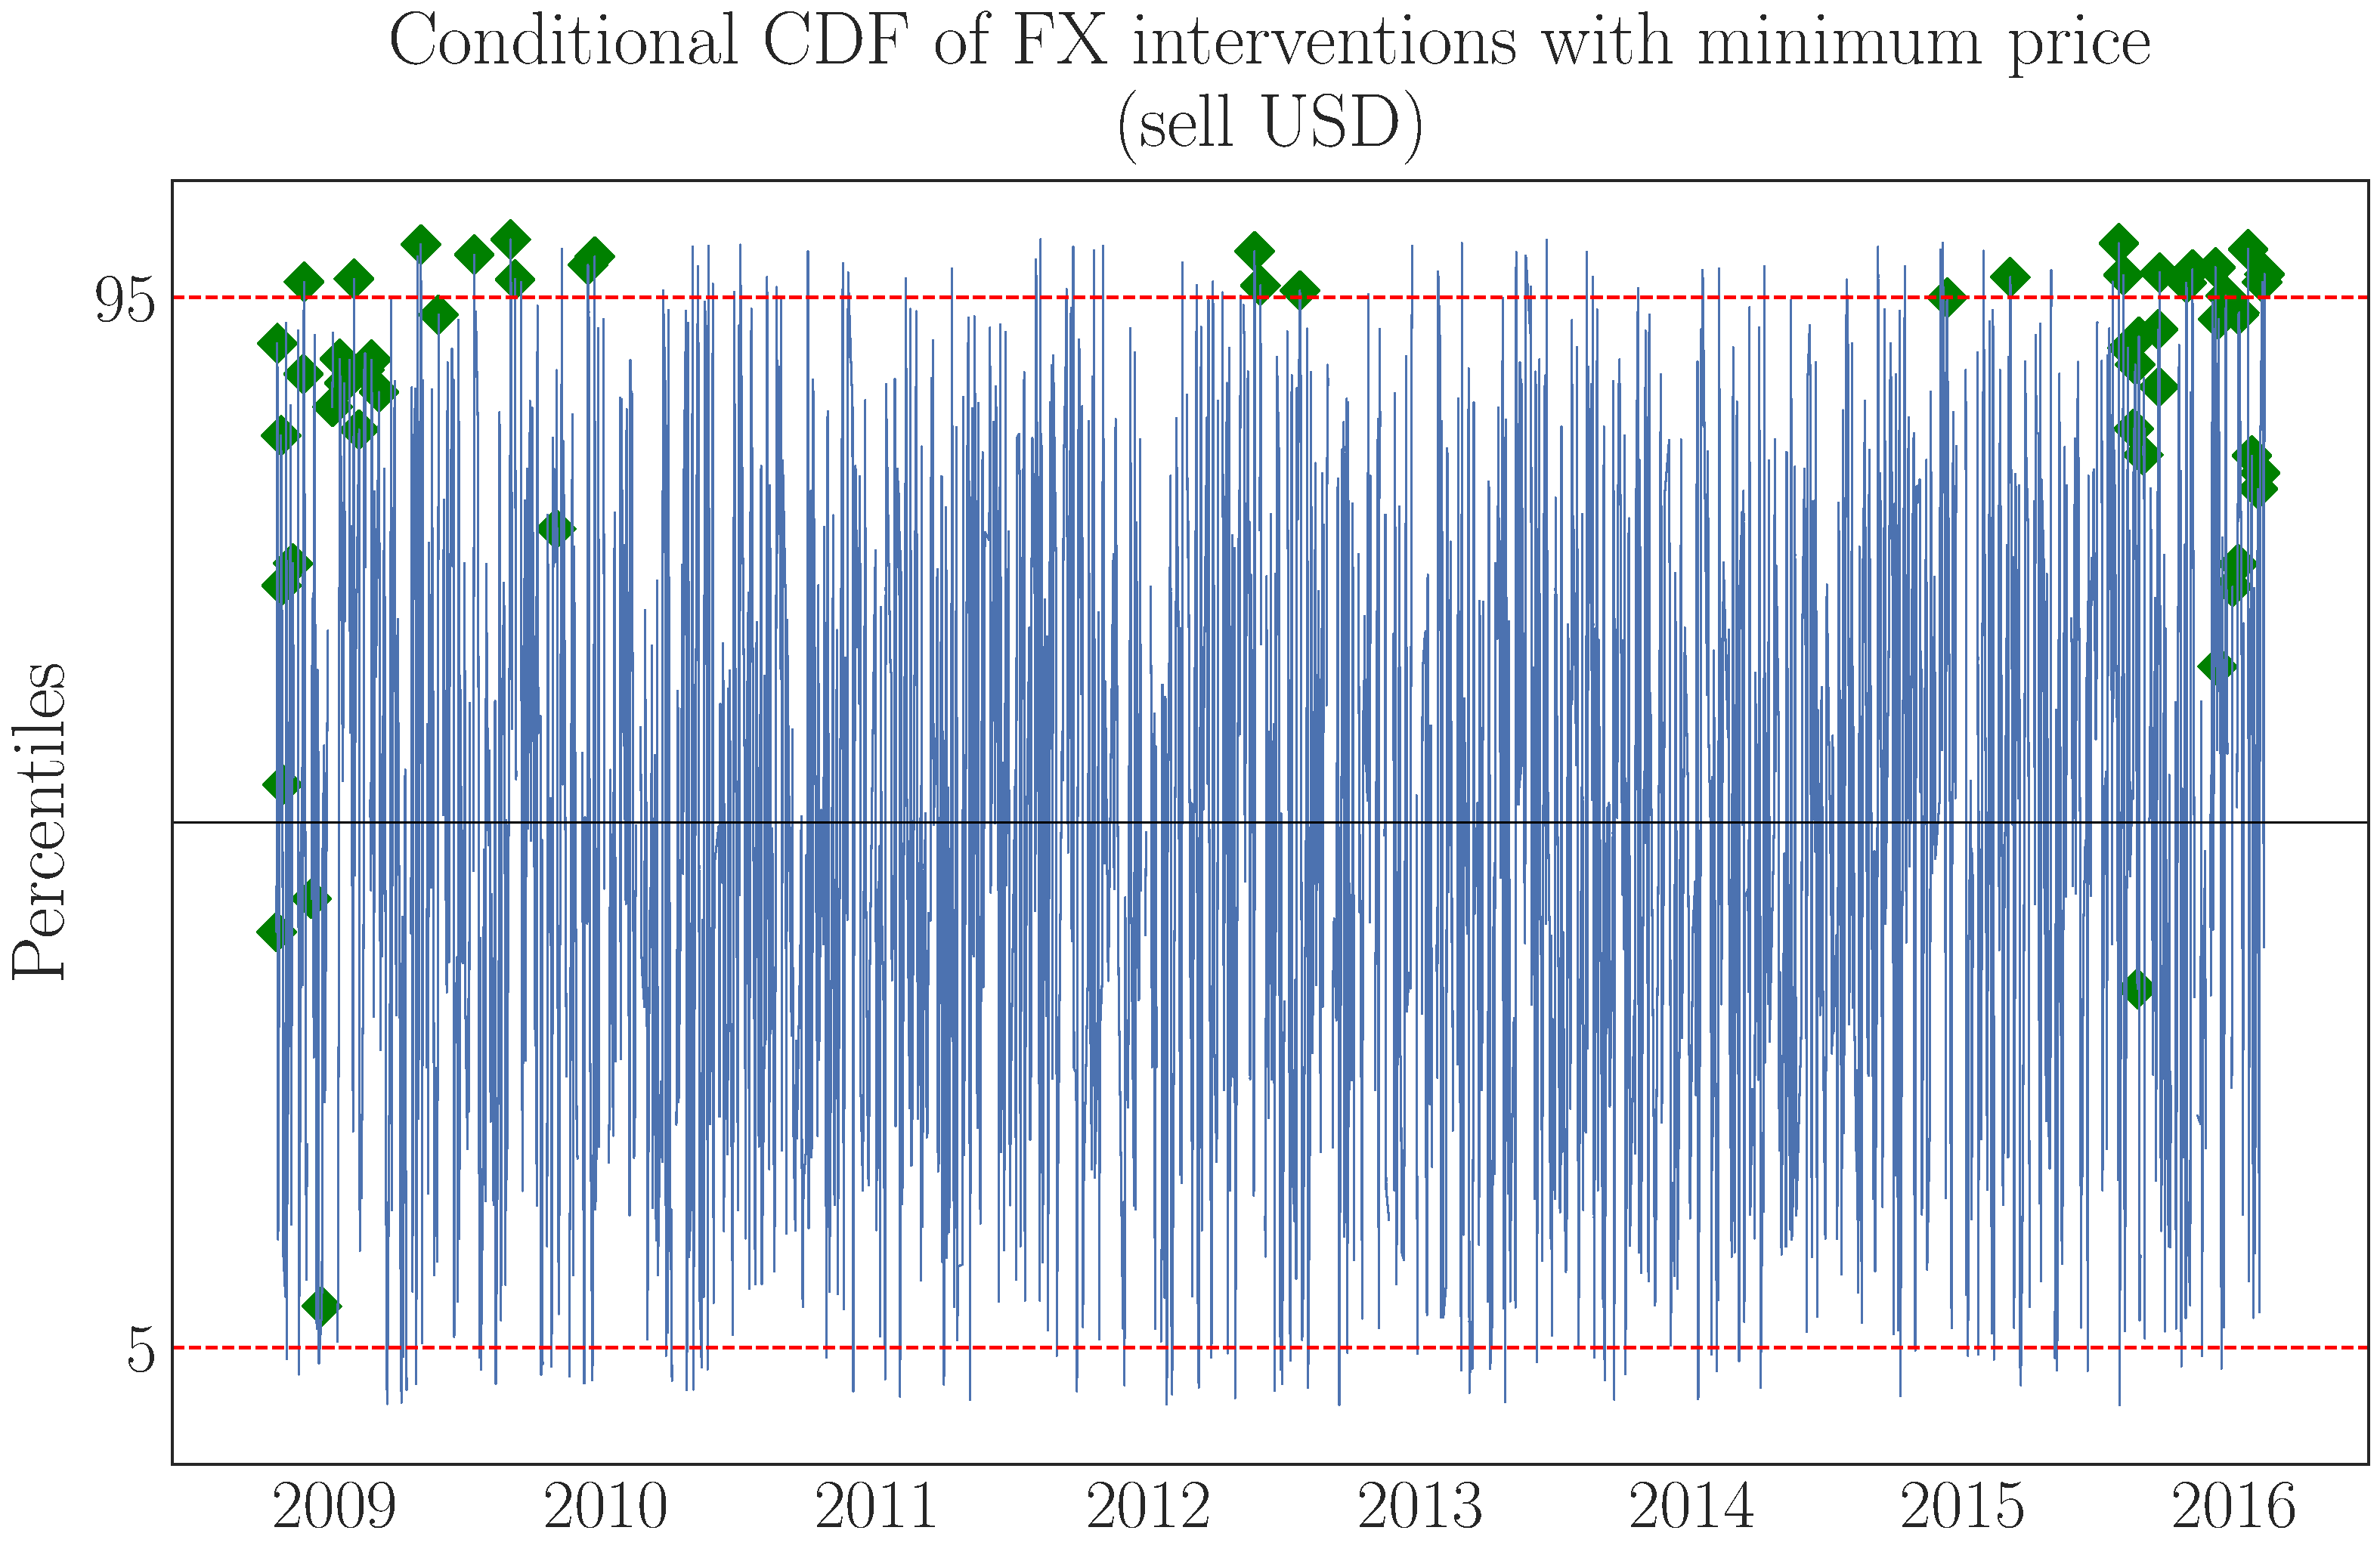
\includegraphics[width=\paperwidth]{benchmark_minprice_cdf.pdf}}
\end{frame}


\begin{frame}
  \frametitle{Discretion-Based Benchmarking}
    \makebox[\linewidth]{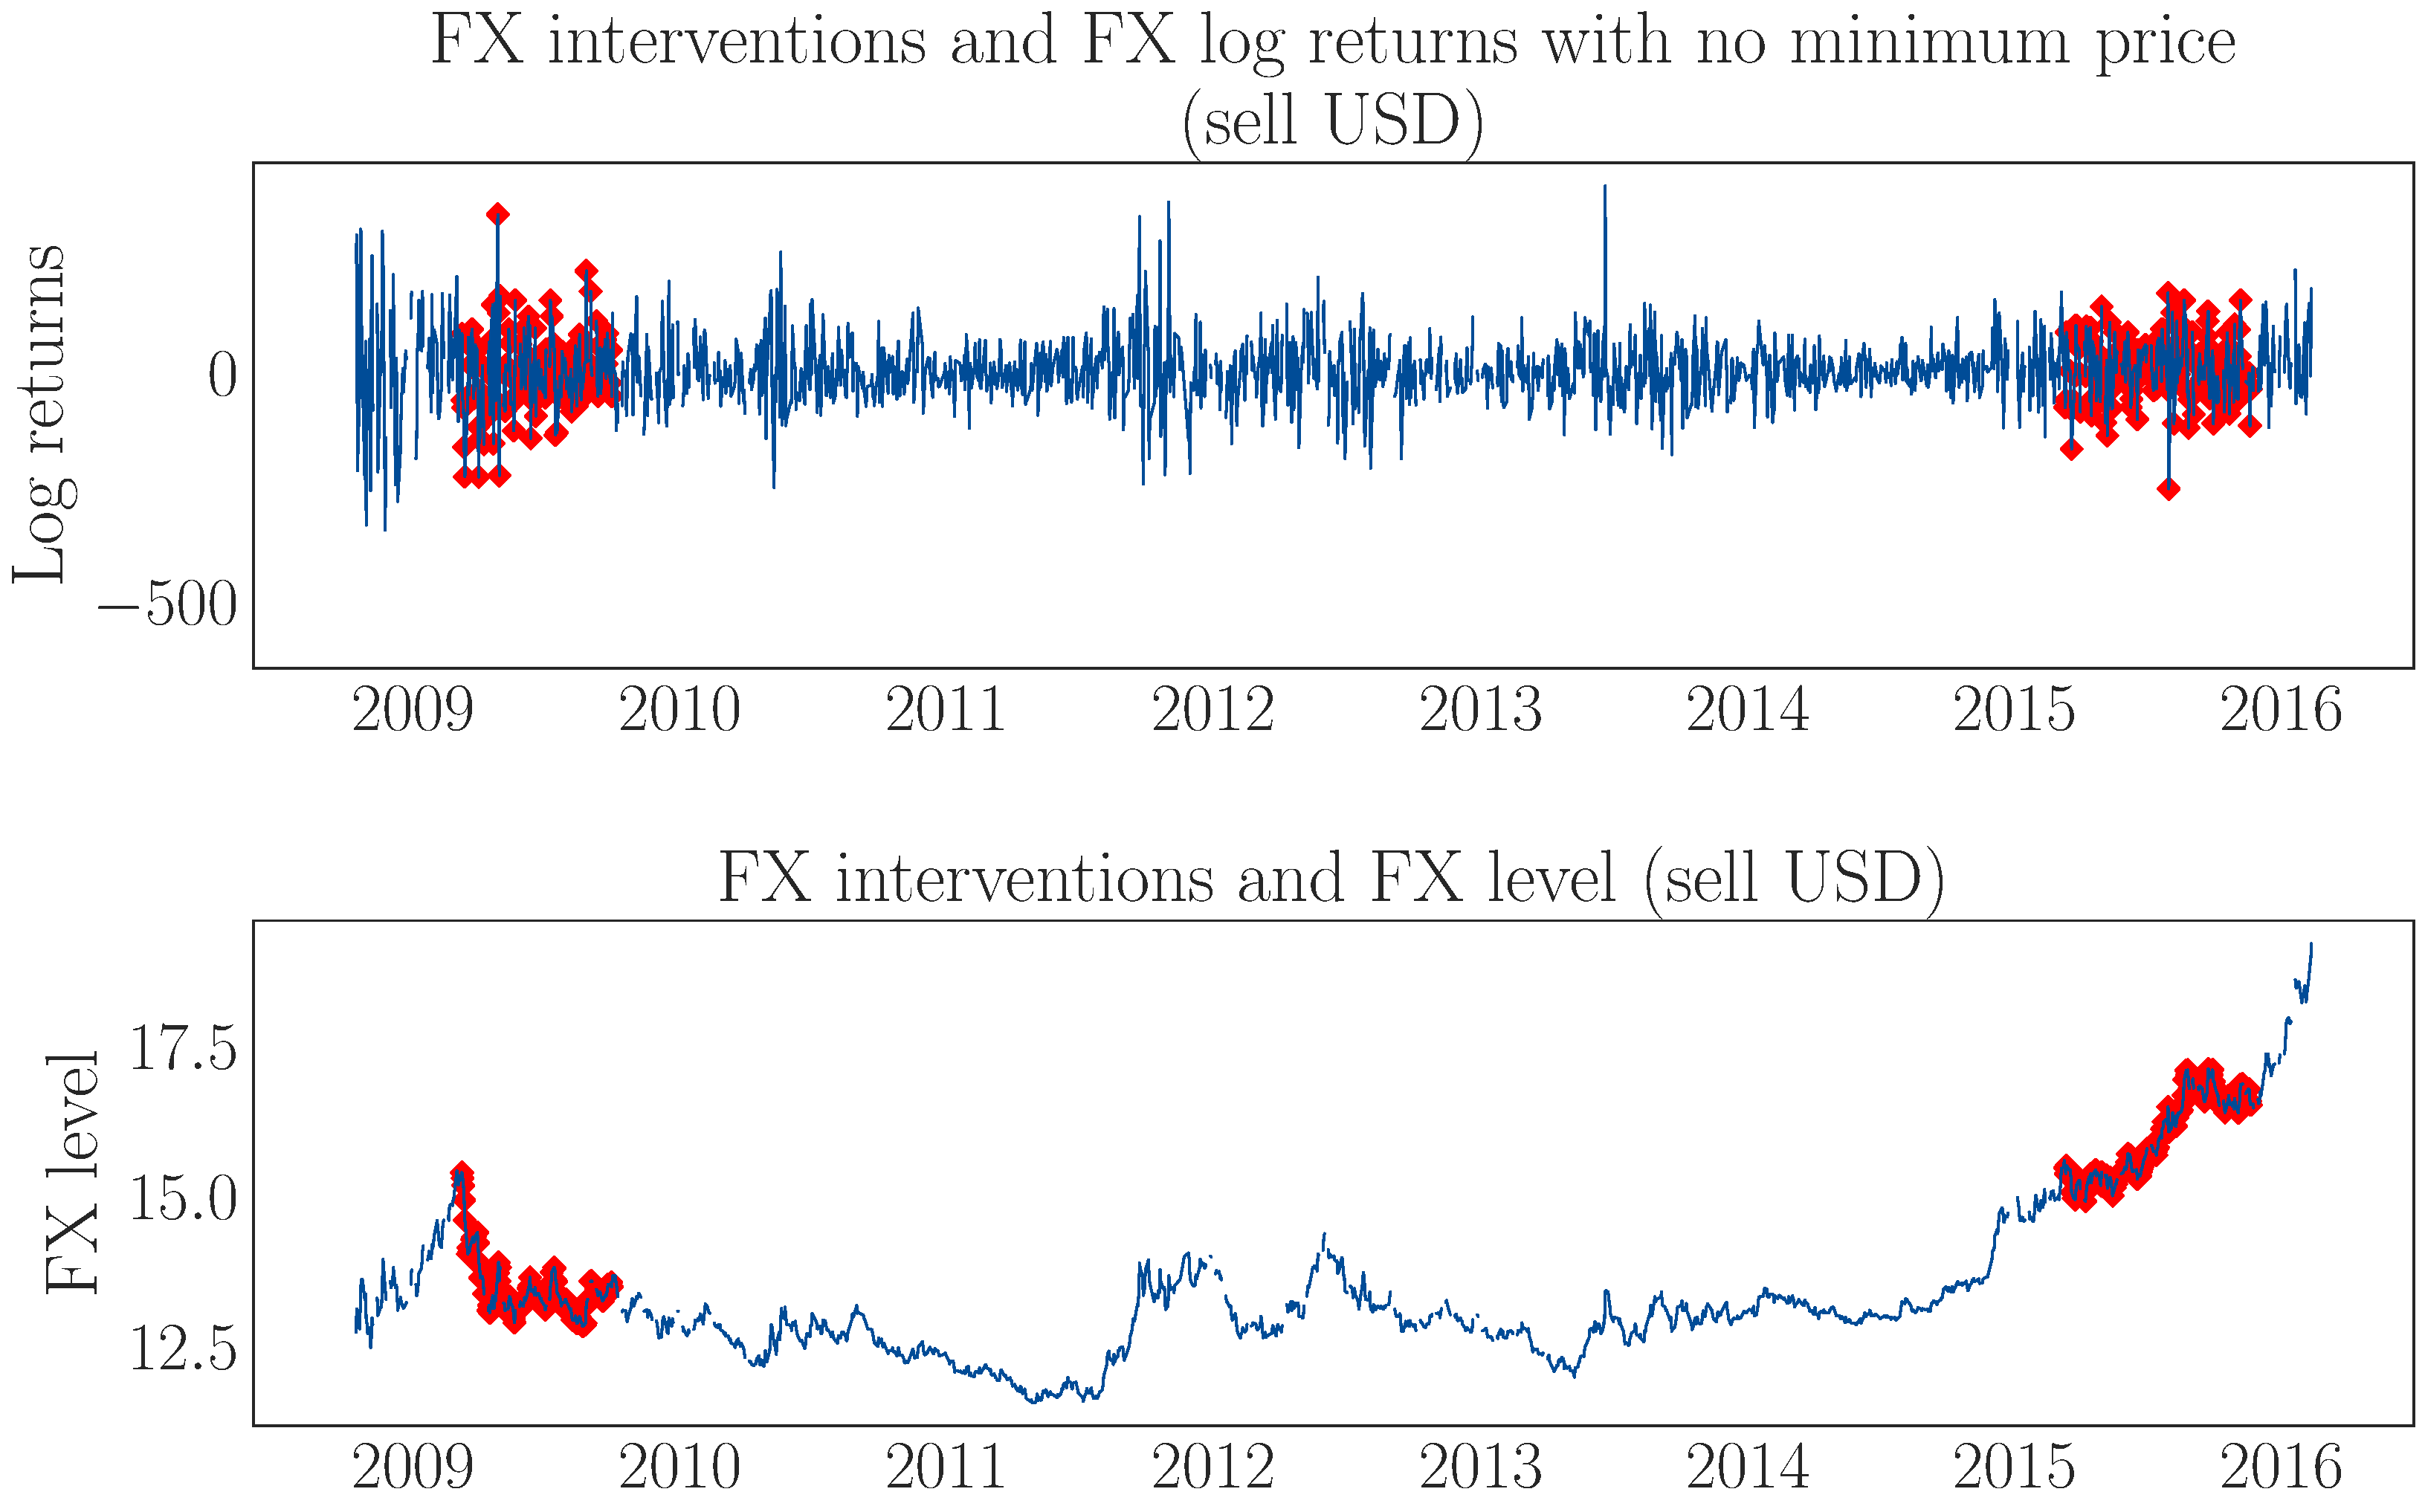
\includegraphics[width=\paperwidth]{benchmark_no_minprice.pdf}}
\end{frame}


\begin{frame}
  \frametitle{Discretion-Based Benchmarking: Risk-Level}
    \makebox[\linewidth]{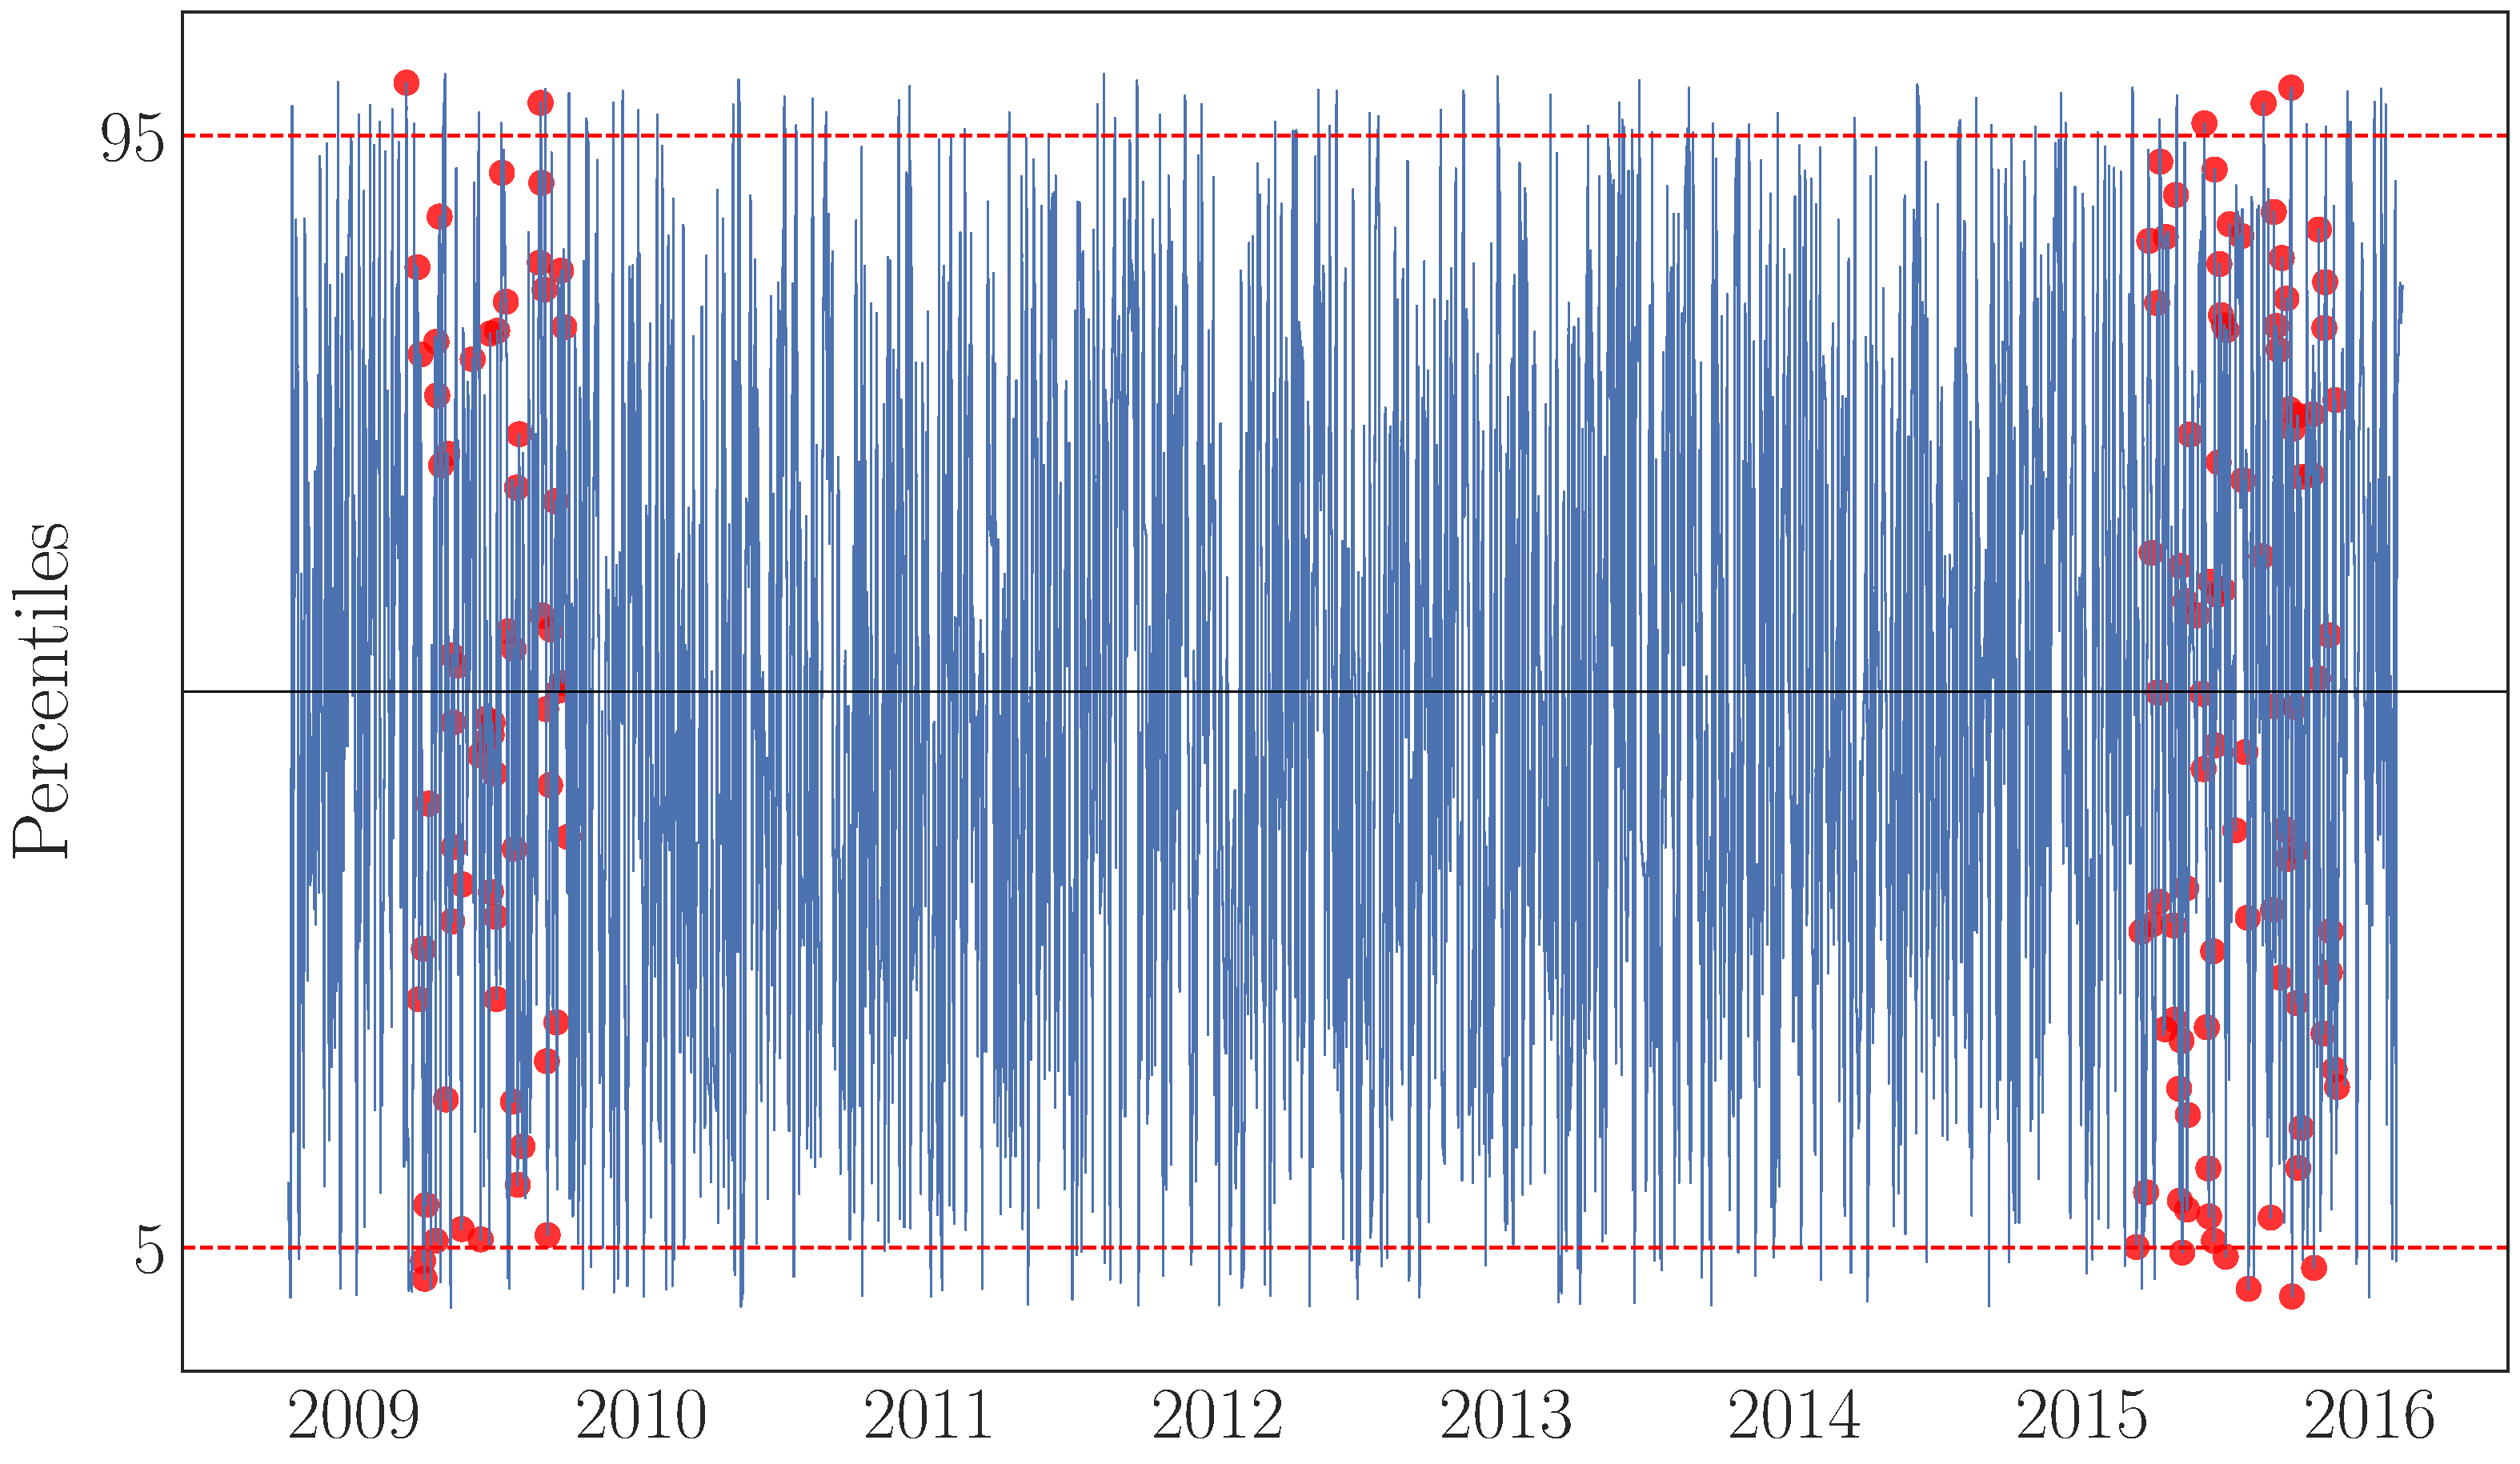
\includegraphics[width=\paperwidth]{benchmark_no_minprice_cdf.pdf}}
\end{frame}



\begin{frame}
  \frametitle{Benchmarking Results}
  \begin{largeitemize}
    \item The fixed volatility rule did not fully prevented BM to intervene
      outside of the tails of the conditional distribution
    \item In that respect, VaR-based intervention would have been better
    \item However, interventions under fixed volatility were significantly
      less frequently outside of the tails than discretionary interventions
    \item \textbf{Discretion triggers are not identifiable based on risk}
  \end{largeitemize}
\end{frame}


%% ---------------------------------------------------------------------------
%% Conclusion
%% ---------------------------------------------------------------------------

\section{Policy Implications and Future Work}

\begin{frame}
  \frametitle{Policy Implications}
  \begin{largeitemize}
   \item Useful for floating rate regimes, where the central bank is concerned with FX
     risks to financial stability
    \item The VaR-based rule could be considered \textbf{as one option} to improve the
      rules that central banks currently use
    \item Let the nominal exchange rate acts as a \textbf{shock absorber}
    \item Could be used to accompany the \textbf{transition to exchange rate
      flexibility}, with gradually less and less interventions
  \item \textbf{Foster the development of hedging markets}
    \item Properly \textbf{fix market incentives
      and anchor expectations}: avoid moral hazard and windfall effects
  \item More generally, could be used by central banks for \textbf{market and risk monitoring}
  \end{largeitemize}
\end{frame}



\begin{frame}
  \frametitle{Future Work}
  \begin{largeenumerate}
    \item Use expected shortfall (ES) instead of VaR, as ES has better risk properties
    
    \item Look \textbf{beyond spot FX markets} and apply a similar and consistent
      approach to:
      \begin{itemize}
      \item FX derivatives, e.g. forward spreads
      \item Offshore/onshore interest
        rate markets
      \item Fixed income market 
      \end{itemize}
   \item Determine the risk tolerance by \textbf{identifying vulnerabilities} and their
     impact to the economy. Align with the "\textbf{at-risk}" work done in MCM
  \end{largeenumerate}
\end{frame}




%% ---------------------------------------------------------------------------
%% End document
%% ---------------------------------------------------------------------------
\end{document}

